%!TEX root = ../physical-olympics-2.tex
\chapter{振动与波}


\section{方程与谐振}

\subsection{简谐振动的定义}
振动是最常见的物理现象.\,而振动中的最简单(simple)而和谐(harmonic)者谓之\emph{简谐振动}(simple harmonic oscillation).\,对\emph{谐振子}(harmonic oscillator)的学习与研究是会贯彻整个物理理论不同层次内容的始终的.\,现在是经典力学,\,以后会上升到场论,\, 量子力学与量子场论的高度.

简谐振动是指一个物理量$Q$随时间围绕其平衡位置做上下的波动.\,其形式符合:
\[Q=Q_0+\Delta Q\cos(\omega t+\varphi)\]

我们经常会有用复数表示振动的习惯,\,其做法是在三角函数$\cos$与其\emph{宗量}(argument)\,$\phi=\omega t+\varphi$构成的项后添加一个虚的$\ui \sin\phi$项,\,于是新的写法变成:
\[\tilde{Q}(t)=Q_0+\Delta Q\ue^{\ui(\omega t+\varphi)}\; ; \; Q=\mathfrak{Re}(\tilde{Q})\]

又或者:
\[\tilde{Q}(t)=Q_0+\Delta \tilde{Q}\ue^{\ui\omega t}\; ; \; \Delta \tilde{Q}=\Delta Q\ue^{\ui\varphi}\]

以上各个常量中,\,$Q_0$是平衡位置,\,$\Delta Q$叫\emph{振幅}(amplitude),\,宗量$\omega t+\varphi$叫做\emph{相位}(phase),\,$\omega$叫\emph{角频率}(angular frequency),\,$\varphi$叫初相位.\,$\tilde{Q}$为复化的复物理量,\,而$\Delta \tilde{Q}$叫做\emph{复振幅}(complex amplitude).

复数表示最大的一个好处就在于很方便计算物理量的线性组合与导数.\,事实上,\,如果合理选取$Q_0=0$:
\[\dot{Q}=-\omega\Delta Q\sin\phi\; ; \; \dot{\tilde{Q}}=\ui\omega\tilde{Q}\quad \Rightarrow\quad \dot{Q}=\mathfrak{Re}(\dot{\tilde{Q}})\]
\[\ddot{Q}=-\omega^2\Delta Q\cos\phi\; ; \; \ddot{\tilde{Q}}=-\omega^2\tilde{Q}\quad \Rightarrow\quad \ddot{Q}=\mathfrak{Re}(\ddot{\tilde{Q}})\]

\subsection{简谐振动的性质}
以一个质点水平坐标$x$围绕$x=0$左右做谐振为例.\,其运动方程写作\footnote{以后我们对物理量和物理量的复化只在必要的时候加以区分,\,看到复数只需要认为省写了取实部这一例常操作罢了.}:
\[x=A\ue^{\ui(\omega t+\varphi)}\]

那么其速度与加速度为:
\[v=\ui\omega A\ue^{\ui(\omega t+\varphi)},\,a=-\omega^2A\ue^{\ui(\omega t+\varphi)}\]

我们发现在运动过程中的任意一个时刻,\,加速度都是指向平衡位置的,\,与偏离平衡位置的位移是成正比的:
\[a=-\omega^2 x\]

而任意一个时刻既然$x$是宗量的余弦函数,\,$v$是正弦函数,\,它们就满足其绝对值大小的``此消彼长''关系\footnote{注意到这里(往下)要避免使用复数,\,因为一个复数的实部平方不会等于其平方的实部$v^2\neq\mathfrak{Re}(\tilde{v}^2)$}:
\[v^2+\omega^2 x^2=\omega^2 A^2\]

相位是很重要的物理概念,\,\emph{相}(phase),\,状态也,\,相位则是一个可以用来表示状态的数.\,反过来,\,我们可以根据物体在一个时刻的状态反过来确定这个时刻的相位.\,如果位移是$x$而振幅为$A$,\,则:
\[\phi=\mathrm{Arcsin}\frac{x}{A}\, ,\,\mathrm{Arcsin}\frac{x}{A}\in \left\{\arcsin\frac{x}{A}+2n\pi|n\in\mathbb{Z}\right\}\cup\left\{\pi-\arcsin\frac{x}{A}+2n\pi|n\in\mathbb{Z}\right\}\]

同理如果已知速度$v$和\emph{速度振幅}(velocity amplitude)\,$\omega A$,\,那么相位为:
\[\phi=\mathrm{Arccos}\frac{v}{\omega A}\, ,\,\mathrm{Arccos}\frac{v}{\omega A}\in \left\{\arccos\frac{v}{\omega A}+2n\pi|n\in\mathbb{Z}\right\}\cup\left\{-\arccos\frac{v}{\omega A}+2n\pi|n\in\mathbb{Z}\right\}\]

相位的取法上具有多值性.\,但是相位随时间的变化我们约定必须是连续的,\,事实上它随时间线性增加.\,也就是说如果前一个状态下相位为$\phi_1$,\,后一个状态下相位为$\phi_2$,\,那么这两个状态间历时:
\[\Delta t=\frac{\phi_2-\phi_1}{\omega}\]

\subsection{简谐振动的判定}

事实上以上的两个关系都可以成为体系做简谐振动的判据,\,它们为:

\begin{itemize}
	\item 线性回复判据:\,如果一个随时间演化的变量的二阶导数正比于变量本身,\,且符号相反,\,可以判断变量做简谐振动:
	\[\ddot{q}=-\omega^2 q\quad \Rightarrow \quad q=A\cos(\omega t+\varphi)\]

	\item 此消彼长判据:\,如果一个随时间演化的变量的一阶导数与自己的正系数平方和为动力学守恒量(一般就是能量).\,可以判断变量做简谐振动:
	\[\dot{q}^2+\omega^2 q^2=\omega^2A^2\quad \Rightarrow \quad q=A\cos(\omega t+\varphi)\]
\end{itemize}

证明如下:

线性回复$\Rightarrow$此消彼长:

首先进行代换:

\[\ddot{q}=\frac{\ud}{\ud t}(\dot{q})=\frac{\ud q}{\ud t}\frac{\ud}{\ud q}(\dot{q})=\frac{\dot{q}\ud\dot{q}}{\ud q}\]

将上式代入$\ddot{q}=-\omega^2 q$:
\[\dot{q}\ud\dot{q}+\omega^2 \cdot q\ud q=\ud(\frac{1}{2}\dot{q}^2+\frac{1}{2}\omega^2 q^2)=0\quad \Rightarrow \quad \dot{q}^2+\omega^2 q^2=C\]

命$A=\sqrt{C/\omega^2}$即得到此消彼长判据.

此消彼长$\Rightarrow$简谐振动:

考虑$\dot{q}$的正根即可,\,负根结果也是简谐振动:
\[\dot{q}=\frac{\ud q}{\ud t}=\omega\sqrt{A^2-q^2}\]
\[\Rightarrow \quad \frac{\ud q}{\sqrt{A^2-q^2}}=\omega \ud t\]

两边同时积分,\,积分常数写到右侧记作$\varphi$,\,得到:
\[-\arccos \frac{q}{A}=\omega t+\varphi \quad \Rightarrow\quad q=A\cos(\omega t+\varphi)\]
\vspace{-0.1cm}


\subsection{小振动}

值得注意的是,\,很多情况下体系的运动并不是严格的简谐振动.\,十分常见的一种情况是\emph{小振动}(small oscillation).\,事实上,\,如果我们研究体系为完整而稳定的一自由度体系,\,广义坐标为$q$,\,而且势能函数$V(q)$存在一个极小值:
\[V'(q_0)=0\quad,\quad V''(q_0)>0\]

那么根据上一章的阐述,\,这个$q_0$就是体系的稳定平衡位置.\,那么,\,任何偏离这个平衡位置的系统运动只要偏离的值足够小,\,即做坐标变换$\delta=q-q_0$为无穷小量,\,那么就一定为简谐振动.\,这是因为势能可以由泰勒展开为:
\[V=\frac{1}{2}V''(q_0)\delta^2+\frac{1}{3!}V'''(q_0)\delta^3+\cdots\]

只要$\delta$足够小,\,三阶项就必然远小于二阶项.\,从而可以只保留第一项.\,同理这也适用于动能,\,它必然正比于$\dot{\delta}$的平方,\,系数则与平衡位置有关:
\[T=\frac{1}{2}M(q_0)\dot{\delta}^2\]

从而这个体系的能量函数(哈密顿量)就被近似为了:
\[H=T+V=\frac{1}{2}M(q_0)\dot{\delta}^2+\frac{1}{2}V''(q_0)\delta^2\]

这就直接符合了``此消彼长''判据.\,从而小振动的角频率为:
\[\omega=\sqrt{\frac{V''(q_0)}{M(q_0)}}\]

例如,\,在典型的单摆问题中,\,取摆线与竖直方向的夹角$\theta$为广义坐标.\,摆球的重力势能以平衡位置为原点表示为:
\[V(\theta)=mgl(1-\cos\theta)\]

而动能为:
\[T=\frac{1}{2}ml^2\dot{\theta}^2\quad \Rightarrow\quad M(\theta)=ml^2\]

从而只需要带入以上公式,\,就得到:
\[\omega=\sqrt{\frac{V''(0)}{M(0)}}=\sqrt{\frac{mgl}{ml^2}}=\sqrt{\frac{g}{l}}\]

这是因为事先看出来了稳定平衡点为$\theta=0$.\,简单的小振动问题的思路都大抵如此.\,第一步是写出能量函数来,\,它决定体系的所有可能的动力学演化.\,第二步要找到稳定平衡位置,\,往往一样地是通过势能函数的增减凹凸性来判断,\,往往也要结合体系的对称性来观察.\,最后便是在平衡位置处把动能势能都近似为简单的平方项.\,唯一需要补充的是,\,除了利用二阶导数来计算这一个平方项,\,对常见函数写泰勒展开式也是十分常见的思路.

单摆问题的周期从而就是:
\[T=\frac{2\pi}{\omega}=2\pi\sqrt{\frac{l}{g}}\]

但是一定要注意这个振动仅仅对小振动成立.\,例如在摆角为$10\dgr=0.087{\rm rad}$时会有约$2\permil$的误差.\,如何计算这个误差?\,之后的非线性振动将讨论这个问题.


\section{阻尼振动与受迫振动}

\subsection{阻尼振动}

阻尼振动,\,狭义地是指普通的弹簧型谐振子,\,但是让振子运动的空间充满介质而产生湿摩擦(流体摩擦).\,从而产生一个正比于速度的阻尼的情形.\,其牛顿定律为:
\[m\ddot{x}=-kx-\gamma \dot{x}\]

这里的$\gamma$即\emph{阻尼系数}(damping coefficient).\,习惯上把$m/\gamma$称作\emph{弛豫时间}(relaxation time).\,最后还定义\emph{衰减参数}(attenuation parameter)或\emph{损耗参数}(loss parameter)为:
\[\beta=\frac{\gamma}{2m}\]

而无阻尼情况下的\emph{固有频率}(natural frequency), 这里是角频率,\,为:
\[\omega_0=\sqrt{\frac{k}{m}}\]

这样原来的方程又被重新写为:
\[\ddot{x}+2\beta \dot{x}+\omega_0^2 x=0\]

我们定义广义的\emph{阻尼振动}(damped oscillation),\,只需要一个运动的任意自由度$q$,\,符合或者可以近似为以上式子形式的动力学方程,\,那么这个自由度上的运动就是一个阻尼振动.\,所有的阻尼振动只有两个常数特征,\,一个是固有角频率,\,一个是损耗的大小.

\vspace{1cm}
阻尼振动的求解需要分为三种情况.\,我们统一猜解:
\[x=A\ue^{\ui\omega t}\]

带入原方程以后发现$\omega$需要满足:
\[\omega^2-2\ui\beta\omega-\omega_0^2=0\]

从而:

\begin{itemize}
	\item \emph{欠阻尼}(underdamped)

	常见的小阻尼情况,\,此时$0<\beta<\omega_0$.\,通过对以上方程求解得到两个含有正虚部的关于虚轴对称的根:
	\[\omega_{1,2}=\ui\beta \pm\sqrt{\omega_0^2-\beta^2}\]

	这样就得到了原阻尼振动方程的通解:
	\[x=\ue^{-\beta t}[A\cos(\sqrt{\omega_0^2-\beta^2}t)+B\sin(\sqrt{\omega_0^2-\beta^2}t)]=C\ue^{-\beta t}\cos(\sqrt{\omega_0^2-\beta^2}t+\varphi)\]

	\begin{figure}[H]
	\centering
	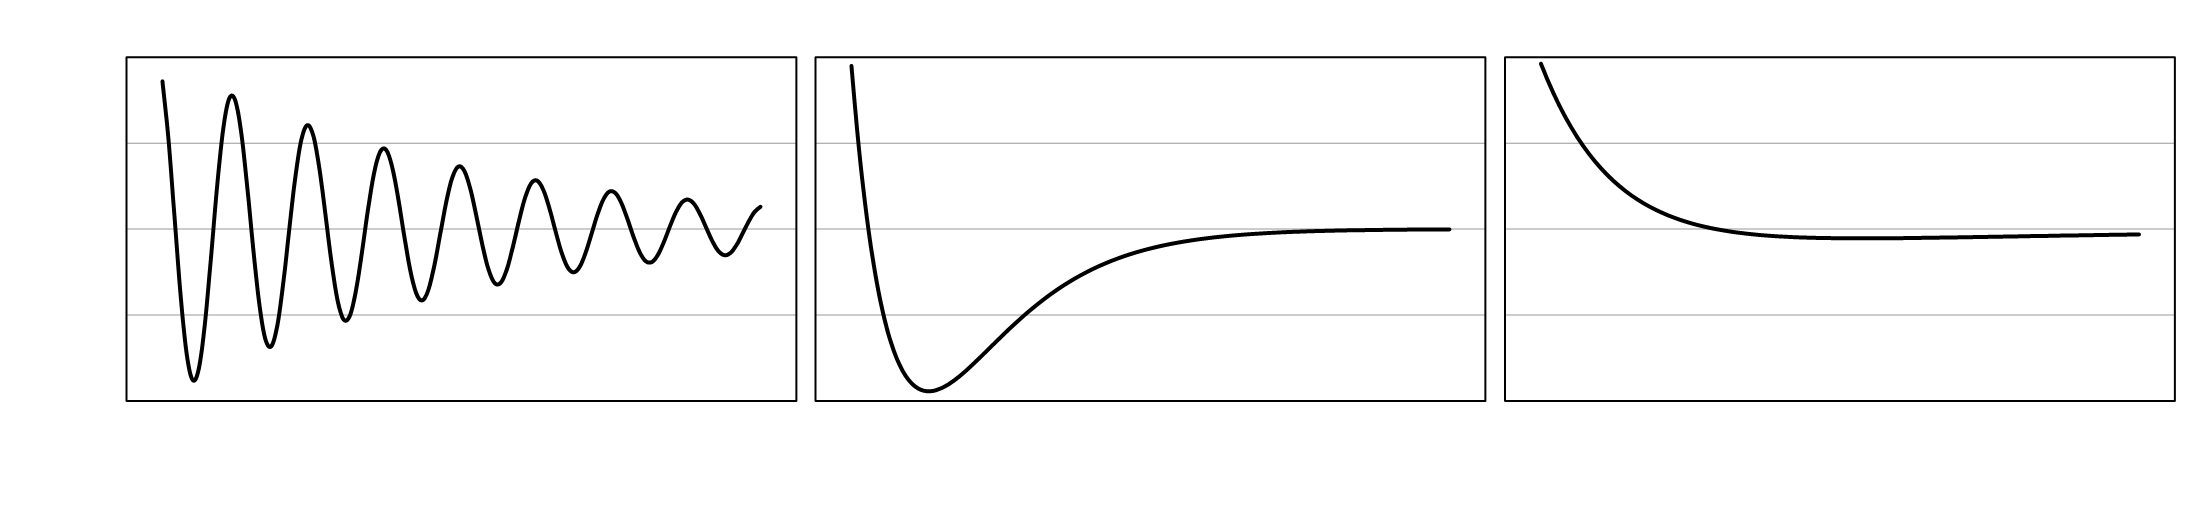
\includegraphics[width=14cm]{image/6-3-1.png}
	\caption{欠阻尼, 临界阻尼与过阻尼}
	\end{figure}

	\item \emph{过阻尼}(overdamped)

	此时$\beta>\omega_0$.\,从而振动和回复力被极大地抑制了.\,主要是一个在大阻力和初速度下缓慢回到平衡位置的运动.\,以上方程两根此时为两个正虚根:
	\[\omega_{1,2}=\ui(\beta\pm\sqrt{\beta^2-\omega_0^2})\]

	这样就得到了原阻尼振动方程的通解:
	\[x=\ue^{-\beta t}[A\ue^{\sqrt{\beta^2-\omega_0^2}t}+B\ue^{-\sqrt{\beta^2-\omega_0^2}t}]=C\ue^{-\beta t}\cosh(\sqrt{\beta^2-\omega_0^2}t+\varphi)\footnote{也有可能是$\sinh$}\]

	\item \emph{临界阻尼}(critical damped)

	这对应$\beta=\omega_0$的特殊情况.\,可以通过微分方程的理论,\,或者采用求$\beta\to \omega_0$极限的方式得到此时的运动方程.\,它为:
	\[x=\ue^{-\beta t}(A+Bt)\]

	临界阻尼在实际生活中的应用为:\,它是较快能够让振子回到平衡位置的理想阻尼大小.\,这一点不难理解,\,不难看出,\,欠阻尼情况的振幅随时间的衰减方式为$\ue^{-\beta t}$,\,也就是适当增大$\beta$有利于振幅尽快衰减.\,但是,\,过阻尼时,\,长时间后位移与时间的关系为
	\[x\sim \ue^{-\beta t}\cosh(\sqrt{\beta^2-\omega_0^2}t)\sim\ue^{-\beta t}\ue^{\sqrt{\beta^2-\omega_0^2}t}\sim \ue^{-\frac{\omega_0^2t}{\beta+\sqrt{\beta^2-\omega^2}}}\]

	这就不难发现,\,此时增加$\beta$只会使得$t$前的衰减系数变小而不利于尽快衰减其位移.\,从而,\,无论是欠阻尼还是过阻尼,\,临界阻尼是它们能够尽快回到平衡位置的极限.\,此时原来的固有频率对应的周期就是它回到平衡位置的特征时间.
\end{itemize}

对于欠阻尼情况,\,尤其是衰减因子$\beta<<\omega_0$的小阻尼情况,\,还有一些重要的性质值得挖掘.\,下面都默认是这样的前提:

\begin{wrapfigure}[17]{o}[-10pt]{7cm}
\centering
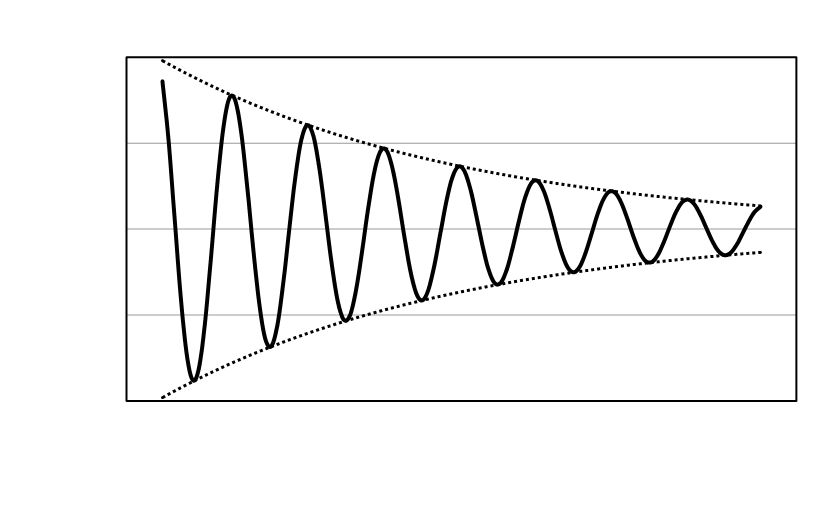
\includegraphics[width=7cm]{image/6-3-2.png}
\caption{\quad 小阻尼下的振幅衰减}
\end{wrapfigure}
从之前的运动方程解不难看出来,\,我们可以把小阻尼情况下的运动方程看作是一个振幅不断随着时间衰减的简谐振动.\,其振幅衰减函数和阻尼化角频率为:
\[A(t)=A_0\ue^{-\beta t}\]
\[\omega_d=\sqrt{\omega_0^2-\beta^2}\approx \omega_0\]

要讨论其衰减的原因,\,还有一种新的角度,\,便是考虑其能量.\,当振幅为$A$时,\,其动能,\,势能的和为:
\[E=T+V=\frac{1}{2}m\dot{x}^2+\frac{1}{2}kx^2\]

现在它不是守恒的,\,仅仅是在少数几个周期里面``近似''守恒.\,但是我们可以考虑求它在一个周期内的平均:
\[\bar{E}=\frac{1}{2}\cdot\frac{1}{2}m\omega_d^2 A^2+\frac{1}{2}\cdot\frac{1}{2} kA^2=\frac{1}{2}m\frac{\omega_0^2+\omega_d^2}{2} A^2\approx \frac{1}{2}m\omega_0^2 A^2\]

现在我们计算单位时间减少的能量的平均值.\,它其实就是阻尼造成的负功功率的平均值:
\[\bar{P}=\overline{\gamma v\cdot v}=\frac{1}{2}\gamma \omega_d^2 A^2\approx \frac{1}{2}\gamma \omega_0^2 A^2=\frac{1}{2}m \omega_0^2 A^2\cdot 2\beta\]

通过损耗功率等于能量的负导数,\,也可以得到振幅随着时间衰减的具体结果.\,我们现在关心一个重要的量,\,它实际上是反应振子振动单位时间所减少的能量占由于以$\omega_0$振动导致的总能量转化速率的比例,\,我们把上式换一种写法:
\[\bar{P}=\frac{\omega_0\bar{E}}{Q}\]

以上引入的$Q$就是著名的\emph{品质因数}(quality factor).\,它越大,\,表示损耗越低,\,振子的阻尼就越小,\,就越接近``谐振''.\,实际上它算法为:
\[Q=\frac{\omega_0}{2\beta}\]

品质因数经常与另一个因子一起提出,\,两者是简单的倒数关系,\,更精确地,\,我们定义:
\[\sin\delta=\frac{1}{2Q}=\frac{\beta}{\omega_0}\]

$\delta$被称作\emph{损耗角}(loss angle).\,一定要注意这两个概念是普遍的.\,谐振子模型是很多实际问题的抽象,\,它们作为谐振子都有自己的品质因数或损耗角,\,用以描述过程的一些共性,\,而且,\,不光可以用能量的损失的共性来定义品质因数和损耗角,\,还有很多重要的方式.\,详情见后.

\begin{wrapfigure}[17]{o}[-10pt]{7cm}
\centering
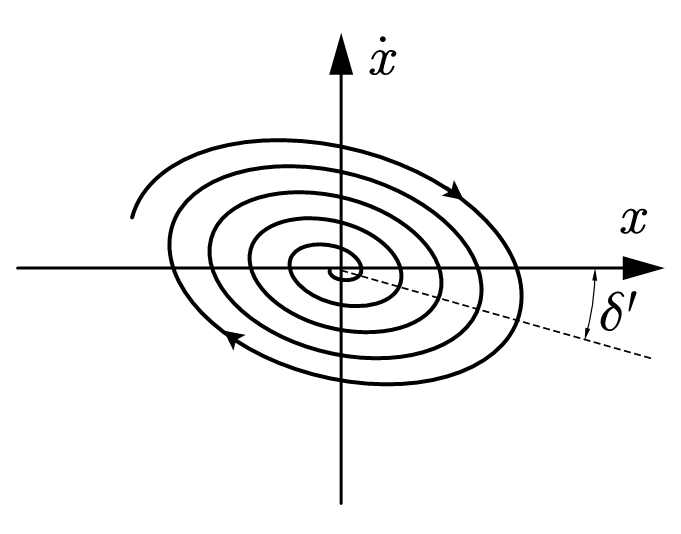
\includegraphics[width=7cm]{image/6-3-3.png}
\caption{阻尼振动的相图}
\end{wrapfigure}
现在我们来考虑简谐振动的\emph{相图}(phase diagram).\,在动力学中,\,这总是指把单个过程的运动,\,画成以其广义坐标和广义速度(或动量)为坐标轴的\emph{相空间}(phase space)中的曲线形成的图像.\,阻尼振动的代表性解为:
\[x=A\ue^{-\beta t}\ue^{\ui \omega_d t}\]

在这个解下,\,其速度为:
\[\dot{x}=(\ui\omega_d-\beta)A\ue^{-\beta t}\ue^{\ui \omega_d t}\]

两个量都在随时间衰减.\,从而在相图上就体现为一随着时间不断向着原点靠近的螺旋线.\,如果没有阻尼,\,那么标准简谐振动的相轨迹就是正椭圆:
\[\frac{x^2	}{A^2}+\frac{\dot{x}^2}{\omega_0^2A^2}=1\]

但是,\,有阻尼时除了是螺旋式的椭圆,\,它还不是``正''的.\,事实上,\,如果去除衰减因子,\,即将$x$和$\dot{x}$乘以个$\ue^{\beta t}$以抵消其衰减:
\[X=x\ue^{\beta t}=A\ue^{\ui \omega_d t}\quad,\quad V=\dot{x}\ue^{\beta t}=\ui(\omega_d+\ui\beta)A\ue^{\ui \omega_d t}\]

两者之间也不是恰好相差相位$\pi/2$,\,而是有一个额外相位差:
\[\delta=\arctan\frac{\beta}{\omega_d}=\arcsin\frac{\beta}{\omega_0}\]

可以发现这个相位差就是损耗角.\,也就是说,\,损耗角的另一种理解方式是位置与速度振动过程中的相位夹角.\,作为结果,\,其相图中的椭圆也要倾斜一个角度$\delta'$.\,可以证明,\,损耗角越大,\,这个倾斜角度也会越大.

\subsection{受迫振动}

如果在谐振子上施加一个周期性的策动外力.\,我们总是研究基本的简谐式的外力\footnote{傅里叶分析理论告诉我们,\,任何函数都可以分解为无穷多助三角函数的线性组合.\,故对于线性系统原则上就可以用叠加原理处理任意任意强迫力的运动求解:\,只要我们把简谐强迫力找到解法.}:
\[F(t)=F_0\ue^{\ui\omega t}\quad {\rm i.e.}\quad F(t)=F_0\cos{\omega t}\]

这个运动就称作\emph{受迫振动}(driven oscillation).\,这样子原来的方程就变为:
\[m\ddot{x}+\gamma\dot{x}+kx=F_0\ue^{\ui\omega t}\]
\[\Rightarrow\quad \ddot{x}+2\beta\dot{x}+\omega_0^2 x=\frac{F_0}{m}\ue^{\ui\omega t}\]

很明显,\,可以猜一个谐振解.\,它是上述微分方程的特解(稳态解).\,通解还需要加上上一部分讨论的阻尼振动解(齐次方程的解是暂态解).\,注意其振动频率应当是策动力的频率$\omega$而不是体系的固有频率$\omega_0$:
\[x=A\ue^{\ui\omega t}\quad \Rightarrow \quad (\omega_0^2-\omega^2+2\ui\beta\omega)A=\frac{F_0}{m}\]

故,\,复振幅的解法也是相当地直接:
\[A=\frac{F_0/m}{\omega_0^2-\omega^2+2\ui\beta\omega}\]


作为复振幅,\,上$A$表达式其实同时包含了两个因素,\,一个是振幅,\,一个是相位.\,现在我们分离它们:
\[A=|A|\ue^{\ui \varphi}\]
\[|A|=\frac{F_0/m}{\sqrt{(\omega_0^2-\omega^2)^2+4\beta^2\omega^2}}\]
\[\varphi=-\arctan\frac{2\beta\omega}{\omega_0^2-\omega^2}\quad {\rm or} \quad \varphi=-\left(\pi-\arctan\frac{2\beta\omega}{\omega^2-\omega_0^2}\right)\]

\begin{wrapfigure}[15]{o}[-10pt]{7cm}
\centering
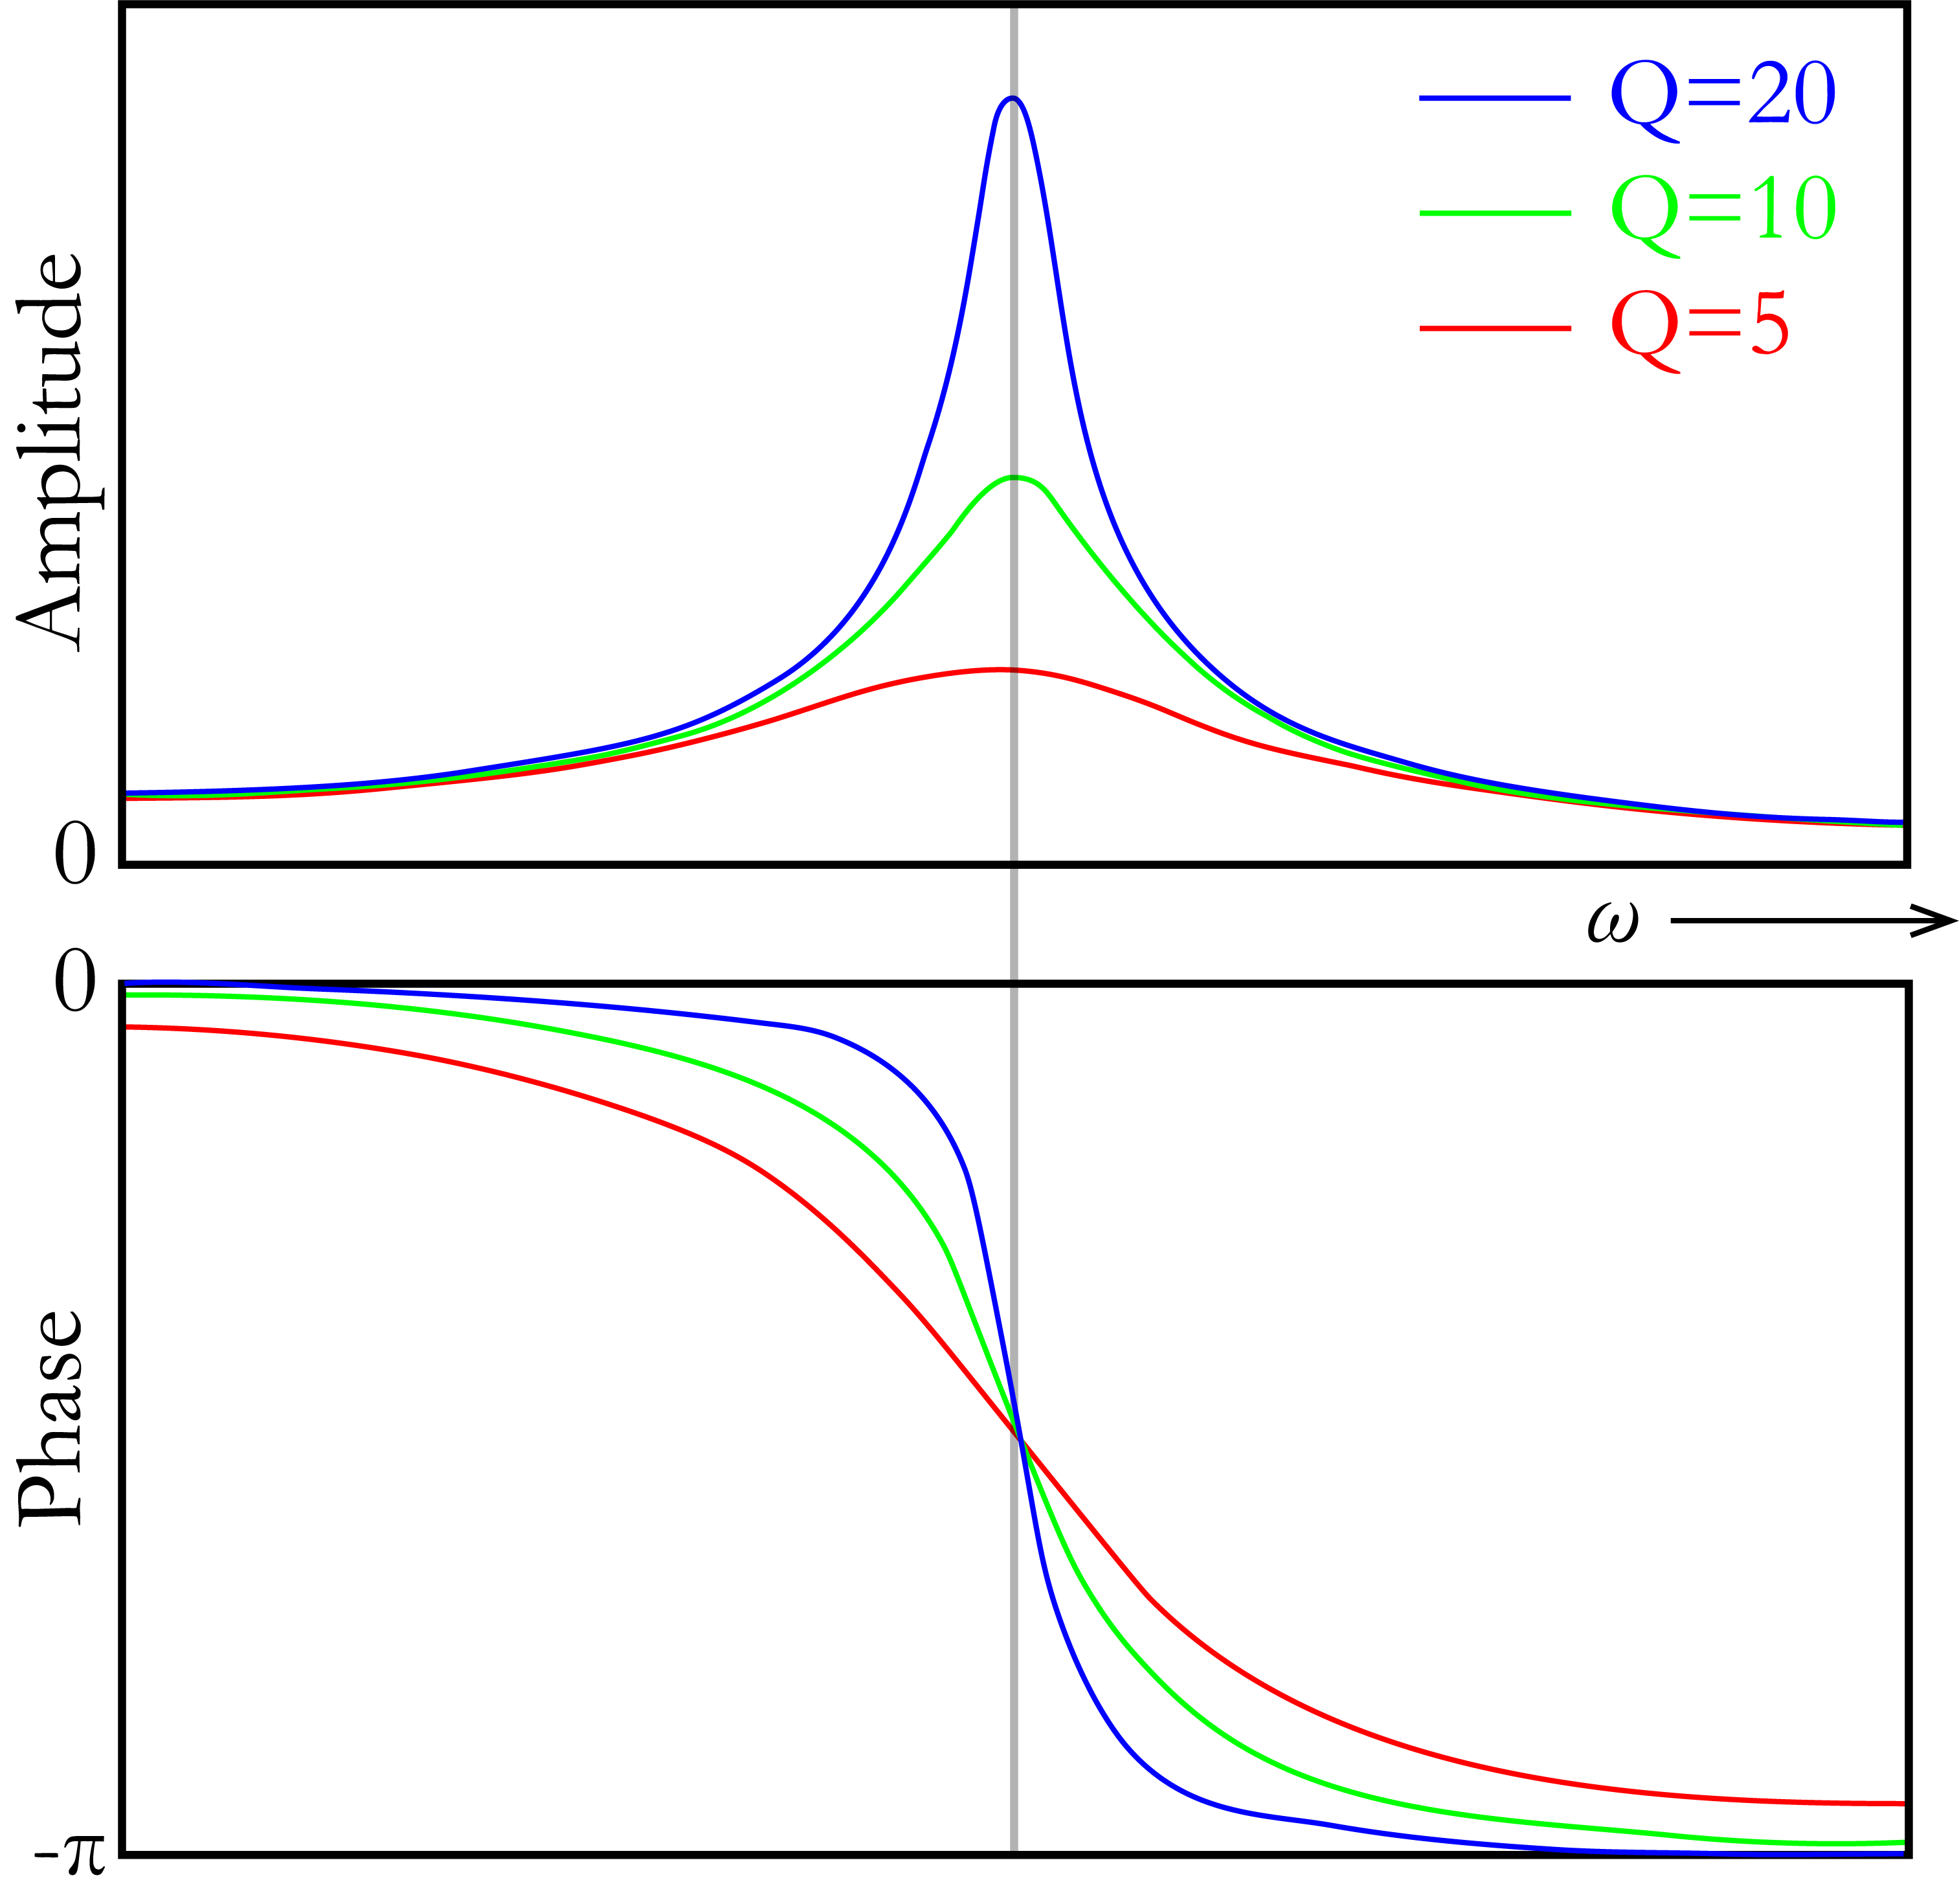
\includegraphics[width=7cm]{image/6-3-4.png}
\caption{幅频, 相频特性}\label{6-3-4}
\end{wrapfigure}
这就构成了两个关于$\omega$的函数.\,这也是实验上我们特别关心的两个函数,\,它们反映在稳态受迫振动的时候,\,一定外力下振子产生的振幅与相位究竟是怎样取决于策动力的角频率的.\,这就是著名的\emph{幅频特性}(amplitude-frequency characteristic)和\emph{相频特性}(phase-frequency characteristic).\,利用之前定义的品质因数$Q$,\,再命$x=\omega/\omega_0$.\,整理得:
\[|A|=\frac{QF_0/m\omega_0^2}{\sqrt{Q^2(1-x^2)^2+x^2}}\]
\[\varphi=-\arccos\frac{Q (1-x^2)}{\sqrt{Q^2(1-x^2)^2+x^2}}\]


我们依然只考虑小阻尼情况.\,此时$Q$较大.\,比如如图\ref{6-3-4}所示,\,$Q=5,\,10,\,20$等.

那么受迫振动又被分为三种情形:

\begin{itemize}
	\item 低频区为弹性控制区.

	在$\omega\ll\omega_0$时,\,$m\ddot{x},\,\gamma\dot{x},\,kx$三项中最后一项最大,\,主要是弹簧的弹性力与策动力去平衡.\,从而体现出以下计算结果:
	\[|A|\approx \frac{F_0}{m\omega_0^2}=\frac{F_0}{k}\]
	\[\varphi\approx 0\]

	也就是策动力与位移几乎同相,\,振子有充分的时间去实现平衡.

	\item 高频区为惯性控制区.

	在$\omega\ll\omega_0$时,\,$m\ddot{x},\,\gamma\dot{x},\,kx$三项中第一项最大,\,主要是高速变化的策动力去直接产生振子加速度.\,从而体现出以下计算结果:
	\[|A|\approx \frac{F_0}{mx^2\omega_0^2}=\frac{F_0}{m\omega^2}\]
	\[\varphi\approx -\pi\]

	也就是策动力与位移几乎反相(亦反向).\,振子``随波逐流'',\,弹性力和阻尼力没有时间跟上策动力的节奏.

	\item 中频区为共振区.

	在$\omega$在$\omega_0$附近,\,即量级接近时.\,三个项$m\ddot{x},\,\gamma\dot{x},\,kx$也量级相当.\,如果把结果画成图\ref{6-3-4}.\,可以发现十分典型的现象是,\,振幅在某频率处取到了极值.\,而相位差(绝对值)在某频率处从小于$\pi/2$增加到大于$\pi/2$.
\end{itemize}

\emph{共振}(resonance)是谐振子系统中十分典型的现象.\,一个共振发生的时候有两个量是值得关注的:

第一个值得关注的共振参数,\,是共振的峰的位置.\,即\emph{共振频率}(resonance frequency).\,但是这个因素又被分为位移共振和速度共振,\,即位移振幅$|A|$最大或者速度振幅最大的角频率值.\,或者可以证明,\,等价的是,\,\emph{振幅共振}(amplitude resonance)和\emph{相位共振}(phase resonance).\,前者指的是响应$x$最大的点:
\[x^2=1-\frac{1}{2Q^2}\approx 1\quad \Rightarrow \quad \omega\approx\omega_0\]

后者则指响应和策动力完全相位差为$\pi/2$的情况:
\[x^2=1\quad \Rightarrow \quad \omega=\omega_0\]

可见两个共振在小阻尼情况下几乎是重合的.\,在振幅共振的情况下,\,振幅最终为:
\[|A|=Q\cdot\frac{F_0}{m\omega_0^2}\cdot\sqrt{\frac{4Q^2}{4Q^2-1}}\approx Q\cdot\frac{F_0}{m\omega_0^2}\]

如果以这个角频率的外力$F_0$直接作用在自由的质点上,\,或者是考虑让一个没有阻尼的振子进行固有振动并使弹簧给振子的力就是$F_0$.\,我们发现振子振幅应当是$F_0/m\omega_0^2$.\,这就是说共振时振幅成为了这个振幅的$Q$倍.\,说明了如果让体系从静止开始,\,自某一时刻开始受到周期性的外力而产生振动,\,如果频率接近固有频率,\,体系会十分反常的振幅越来越大,\,直到振幅是自由振幅的$Q$倍.\,这也是品质因数的第二种理解方式:\,共振的放大倍数.

在看相位共振时的策动力-相位差为$\pi/2$的现象.\,这说明了什么?\,这说明策动力与速度完全就是同相的.\,带入$x=1$容易计算此时位移振幅为$|A|=QF_0/m\omega_0^2$,\,等效地可以写成$F_0=m\omega_0^2|A|/Q$.\,那么速度振幅就是$\omega_0|A|$.\,从而策动力对速度单位时间做的功就是:
\[W=\overline{F(t)\dot{x}(t)}=\frac{1}{2}F_0\omega_0|A|=\left.\frac{1}{2}m\omega_0^3|A|^2\right/ Q\]

这与上一部分得到了相似的结果.\,因为振动的能量其实就是:
\[\bar{E}=\frac{1}{2}m\omega_0^2|A|^2\]

也就是说品质因数反映了耗散的能量与总能量(动能势能互相转换)的比例:
\[Q=\frac{\omega_0 \bar{E}}{W}\]

第二个值得关注的共振参数,\,是共振的峰的宽度.\,谐振子模型给出的幅频曲线,\,与著名的\emph{柯西分布}(Cauchy distribution)对应的函数曲线有密切联系,\,柯西分布又常常因为在理论物理学中的广泛使用而称作\emph{洛伦兹型}(lorentzian shape)\footnote{比如谱线的形状,\,即线型,\,就常被视作洛伦兹线型.}.\,所谓柯西分布最初来自概率分布模型,\,它是指以下分布函数:
\[{\rm pdf.}\footnote{probability distribution function,\,即概率分布函数的缩写.}=\frac{1}{\pi[\gamma^2+(x-x_0)^2]}\]

\begin{figure}[H]
\centering
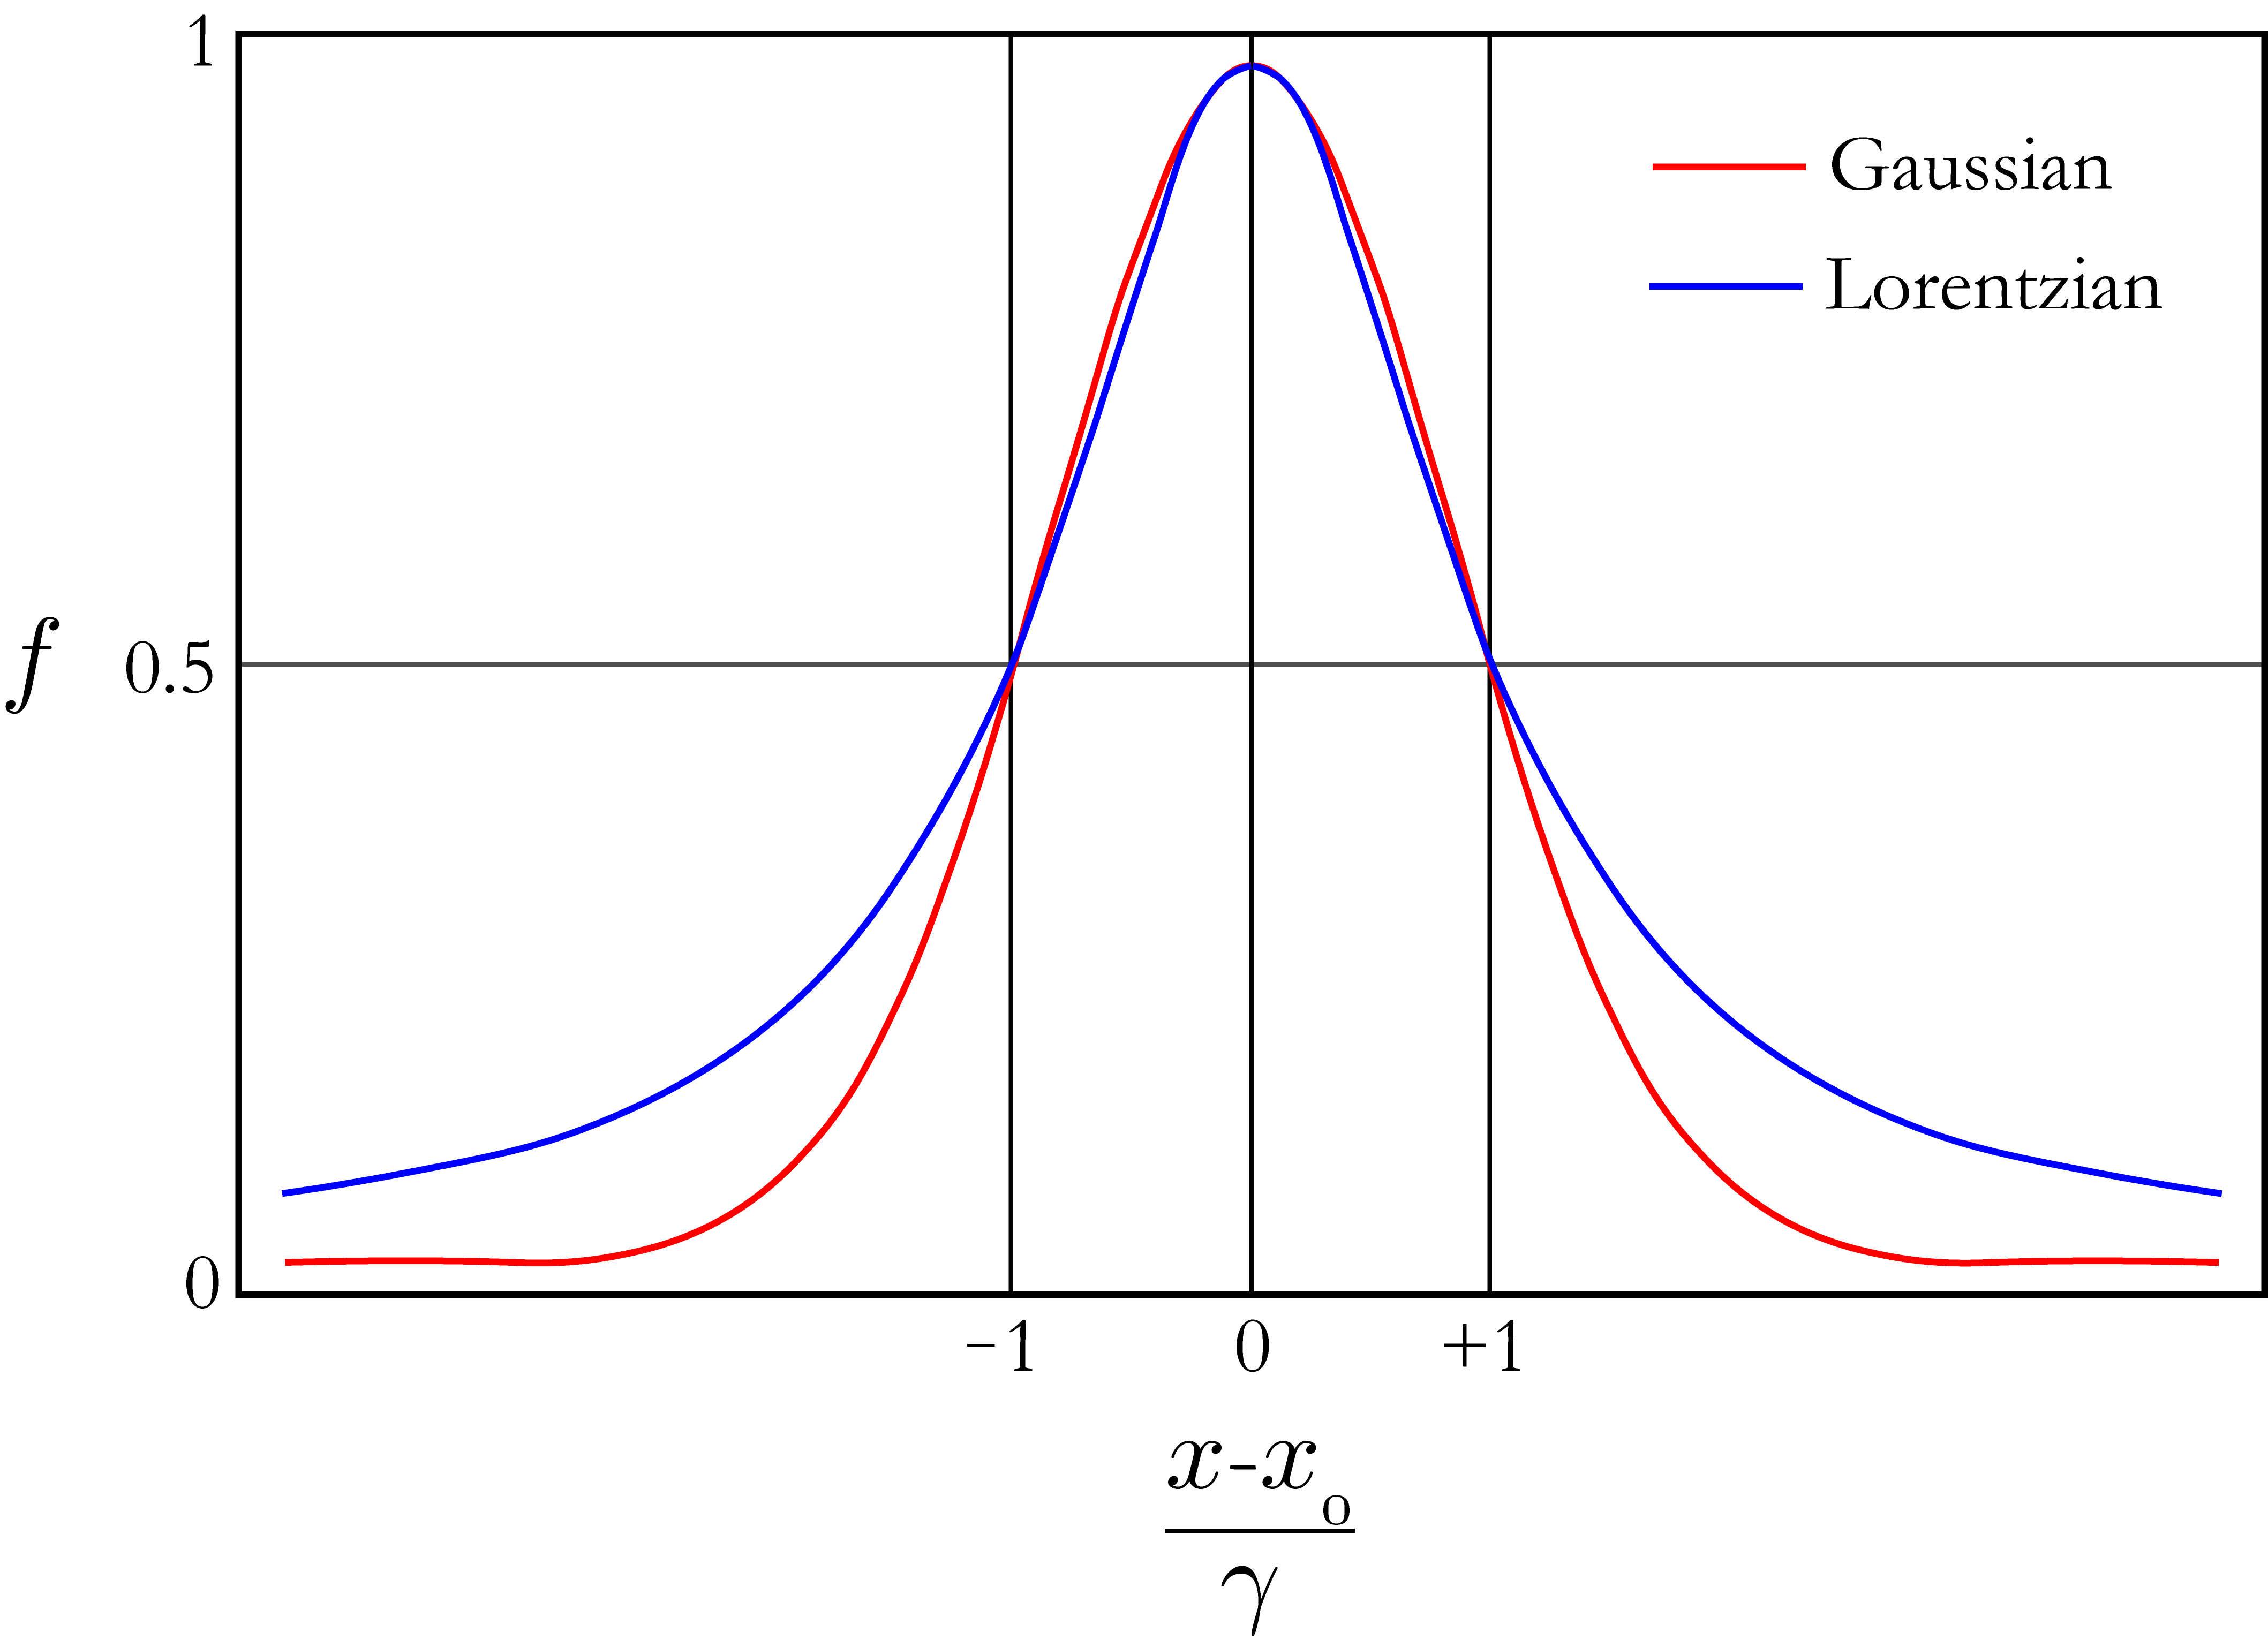
\includegraphics[width=10cm]{image/6-3-5.png}
\caption{高斯型和洛伦兹型\protect\footnotemark}

\end{figure}

\footnotetext{高斯型是指高斯分布:
\[{\rm pdf.}=\frac{1}{\sqrt{2\pi}\sigma}\ue^{-\frac{(x-x_0)^2}{2\sigma^2}}\]}

这样一个分布函数是需要有归一化的要求的:
\[\int_{-\infty}^{+\infty}{\rm pdf. }\,\ud x=1\]

但是现在的幅频特性,\,明显与洛伦兹型是有出入的.\,第一是,\,我们需要把因变量修改为$I=|A|^2$而不是$|A|$.\,这代表振动的强度而不是振幅.\,第二是,\,不同于柯西分布的分母为二次函数,\,这里的分母却作为了$x$的四次函数.\.也是$\omega$的四次函数.\,虽然$I(\omega)$与柯西分布有别,\,而且也不归一化.\,但是却体现出类似的性质.\,它们都是有一个峰,\,并在峰两侧按照较慢的多项式的方式衰减(而不是像高斯型那样指数衰减).\,而且我们都用\emph{半高峰宽}(FWHM,\,full width at half maximum)来描述峰的宽度.\,它被定义为函数值,\,或者代表的强度减少为峰值的一半对应的两点之间的区间宽度.\,对于标准的洛伦兹型,\,容易发现半高峰宽就是:
\[{\rm FWHM}=2\gamma\]

谐振子的幅频曲线的半高峰宽就更加难算.\,我们此时会采取一个近似技巧,\,不难验证其正确性.\,注意到在洛伦兹型中取到半高的点处分母中的两项是相等的,\,于是有理由相信在$I(x)$函数情况下,\,直接让分母两项相等就也近似是在半高点处:
\[I(x)=I_0\left/\middle[(1-x^2)^2+\frac{x^2}{Q^2}\right]\quad\Rightarrow\quad I_{\rm max}\approx I_0\]
\[I=\frac{I_{\rm max}}{2}\quad\Rightarrow\quad 1-x^2\approx \pm\frac{x}{Q}\]

这就可以确定,\,取到半高的点$x_+,\,x_-$为:
\[x_+=\sqrt{1+\frac{1}{4Q^2}}+\frac{1}{2Q}\quad;\quad x_-=\sqrt{1+\frac{1}{4Q^2}}-\frac{1}{2Q}\quad\Rightarrow \quad x_+-x_-=\frac{1}{Q}\]



而$\omega_+=x_+\omega_0,\,\omega_-=x_-\omega_0$.\,从而半高峰宽就是:
\[{\rm FWHM}=\Delta\omega=\omega_+-\omega_-=\frac{\omega_0}{Q}\]

我们又发现了品质因数的一种常见定义方式,\,它被定义为谱线的\emph{锐度}(sharpness),\,即峰处角频率与半高峰宽的比值:
\[Q=\frac{\omega_0}{\Delta \omega}\]





\section{多自由度小振动*}

多自由度小振动,\,首先得是一个多自由度平衡问题.\,在上一章带约束的完整系统的静力学平衡的基础上.\,如果体系还存在$f$个自由度,\,与之对应的有$f$个广义坐标$q_i$.\,那么我们指出过,\,体系的平衡条件为:
\[Q_i=\sum_k \bs{F}_k\cdot \frac{\partial \bs{r}_k}{\partial q_i}=0\]

但是在绝大多数情况下,\,我们处理的是保守体系的问题.\,所以这种场合下又有势能函数$V(q_i)$.\,广义力也能从势能中得到:
\[Q_i=\frac{\partial V}{\partial q_i}\]

这完全就能得到保守体系的平衡条件:
\[\frac{\partial V}{\partial q_i}=0\]

又是在绝大多数情况下,\,势能函数是性质非常良好的函数\footnote{数学上叫做光滑函数.}.\,从而可以在平衡位置附近泰勒展开.\,把平衡位置记作$q_{i0}$,\,而偏离平衡位置的位移为$\delta_i$,\,平衡位置处势能记作$V_0=V(q_{i0})$,\,由于平衡位置一阶导数为零,\,故:
\[V(q_{i0}+\delta_i)=V_0+\frac{1}{2}\sum_{i,\,j}\left.\frac{\partial^2 V}{\partial q_i\partial q_j}\right|_{q_{i0}}\delta_i\delta_j+\frac{1}{3!}\sum_{i,\,j,\,k}\left.\frac{\partial^3 V}{\partial q_i\partial q_j\partial q_k}\right|_{q_{i0}}\delta_i\delta_j\delta_k+\cdots\]

在忽略三阶小量(不会成为领头项,\,条件下面再讨论)的前提下,\,再通过去掉常数$V_0$,\,不影响势能的效果.\,我们发现势能实际上就成为了一个二次型:
\[V=\frac{1}{2}\sum_{i,\,j}\left.\frac{\partial^2 V}{\partial q_i\partial q_j}\right|_{q_{i0}}\delta_i\delta_j=\frac{1}{2}\sum_{i,\,j} V_{ij}\delta_i\delta_j\]

而动能,\,由于在平衡位置附近小范围内做小的运动,\,当然也是一个关于广义速度的二次型,\,系数为常数$T_{ij}$:
\[T=\frac{1}{2}\sum_{i,\,j} T_{ij}\dot{\delta}_i\dot{\delta}_j\]

关于系数$T_{ij},\,V_{ij}$.\,一个要求是它们必须对称:
\[T_{ij}=T_{ji}\quad;\quad V_{ij}=V_{ji}\]

其中的道理非常简单,\,例如只有两个广义坐标的变化$\delta_1,\,\delta_2$.\,那么$V_{12}=a\neq V_{21}=b$所决定的势能二次型与$V_{12}=V_{21}=(a+b)/2$决定的二次型根本就是同一个:
\[V_{12}=a\neq V_{21}=b:\,V=\frac{1}{2}V_{11} \delta_1^2+\frac{1}{2}V_{22} \delta_2^2+\frac{1}{2}a\delta_1\delta_2+\frac{1}{2}b\delta_2\delta_1=\frac{1}{2}V_{11} \delta_1^2+\frac{1}{2}V_{22} \delta_2^2+\frac{1}{2}(a+b)\delta_1\delta_2\]
\[V_{12}=V_{21}=\frac{a+b}{2}:\,V=\frac{1}{2}V_{11} \delta_1^2+\frac{1}{2}V_{22} \delta_2^2+\frac{1}{2}\frac{a+b}{2}\delta_1\delta_2+\frac{1}{2}\frac{a+b}{2}\delta_2\delta_1=\frac{1}{2}V_{11} \delta_1^2+\frac{1}{2}V_{22} \delta_2^2+\frac{1}{2}(a+b)\delta_1\delta_2\]

反过来,\,如果给一个二次型,\,我们也中总可以把系数写成对称的形式,\,比如在动能中,\,毕竟偏导数本身也是可交换次序的:
\[T_{ij}=\frac{\partial^2 T}{\partial \dot{\delta}_i\partial \dot{\delta}_j}=\frac{\partial^2 T}{\partial \dot{\delta}_j\partial \dot{\delta}_i}=T_{ji}\]

\begin{wrapfigure}[38]{o}[-10pt]{6cm}
\centering
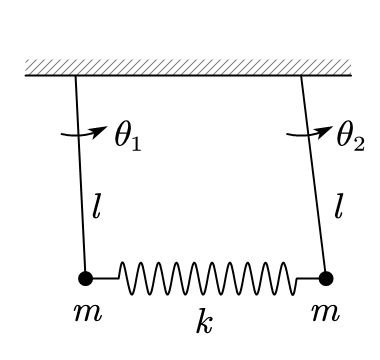
\includegraphics[width=6cm]{image/6-3-7.png}
\caption{耦合摆}\label{6-3-6}
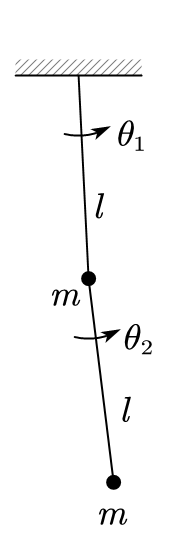
\includegraphics[width=2.5cm]{image/6-3-6.png}
\caption{双摆}\label{6-3-7}
\end{wrapfigure}
举两个例子.\,在\emph{耦合摆}(coupled pendulum)问题\ref{6-3-6}中,\,分开看是相同的两个单摆,\,但却因为弹簧而发生弱的耦合,\,设想弹簧原长为$x$为摆间距,\,这样就使得两单摆按原来的位置平衡时,\,弹簧也没有作用力.\,但只要一发生运动就彼此影响,\,设两摆球距离$x'=\sqrt{(x+l\sin\theta_2-l\sin\theta_1)^2+(l\cos\theta_2-l\cos\theta_1)^2}$.\,这样作为整体体系动能和势能为:
\[T_{\rm cp}=\frac{1}{2}ml^2\dot{\theta}_1^2+\frac{1}{2}ml^2\dot{\theta}_2^2\]
\[V_{\rm cp}=mgl(1-\cos\theta_1)+mgl(1-\cos\theta_2)+\frac{1}{2}k(x'-x)^2\]

再引入描述耦合强度的参量$\varepsilon=kl/mg$,\,小量近似以后,\,动能,\,势能被近似为二次型:
\[T_{\rm cp}=\frac{1}{2}\cdot ml^2\cdot \dot{\theta}_1^2+\frac{1}{2}\cdot ml^2\cdot \dot{\theta}_2^2\]
\[V_{\rm cp}=\frac{1}{2}\cdot (1+\varepsilon)mgl\cdot{\theta}_1^2+\frac{1}{2}\cdot (1+\varepsilon)mgl\cdot{\theta}_2^2-\varepsilon mgl\cdot {\theta}_1{\theta}_2\]

而在\emph{双摆}(double pendulum)问题\ref{6-3-7}中,\,两个摆直接悬挂在一起.\,也会彼此影响.\,体系动能和势能为:
\[T_{\rm dp}=\frac{1}{2}ml^2\dot{\theta}_1^2+\frac{1}{2}ml^2[\dot{\theta}_1^2+\dot{\theta}_2^2+2\dot{\theta}_1\dot{\theta}_2\cos(\theta_1-\theta_2)]\]
\[V_{\rm dp}=mgl(1-\cos\theta_1)+mgl(1-\cos\theta_1)+mgl(1-\cos\theta_2)\]


小量近似以后,\,动能,\,势能被近似为二次型:
\[T_{\rm dp}=\frac{1}{2}\cdot 2ml^2\cdot\dot{\theta}_1^2+\frac{1}{2}\cdot ml^2\cdot\dot{\theta}_2^2+ml^2\cdot\dot{\theta}_1\dot{\theta}_2\]
\[V_{\rm dp}=\frac{1}{2}\cdot 2mgl\cdot{\theta}_1^2+\frac{1}{2}\cdot mgl\cdot{\theta}_2^2\]

如果把$T_{ij}$和$V_{ij}$写成矩阵,\,那么对应的矩阵叫做\emph{惯性矩阵}(inertial matrix)和\emph{弹性矩阵}(elastic matrix):
\[[T_{ij}]_{\rm cp}=ml^2\begin{bmatrix} 1&0\\ 0&1\end{bmatrix}\quad;\quad [V_{ij}]_{\rm cp}=mgl \begin{bmatrix} 1+\varepsilon&-\varepsilon\\ -\varepsilon &1+\varepsilon\end{bmatrix}\]
\[[T_{ij}]_{\rm dp}=ml^2\begin{bmatrix} 2&1\\ 1&1\end{bmatrix}\quad;\quad [V_{ij}]_{\rm dp}=mgl \begin{bmatrix} 2&0\\ 0&1\end{bmatrix}\]

从而我们可以发现这两个问题的重大区别在于,\,前一个问题动能规整,\,势能却具有交叉项.\,后一个问题势能规整,\,动能却具有交叉项.

当我们遇到一个这样普遍的小振动问题时,\,该如何得到其运动的特征.\,有两种常见的做法:\,一是通过换元来实现动能势能的简化,\,这种方法需要较深厚的数学基础,\,又最好通过拉格朗日方程来理解一些过程.\,我们下面也写出具体的过程,\,有兴趣的读者可以做进一步研究;\,但也有第二种简易的方法来求解一些直接的量.\,我们也在详细讨论的方法之后加上去:

\subsection{基于线性代数与分析力学的简正坐标求解}

对一个任意的二次型进行配方并不是难事.\,例如$F(x_1,\,x_2\cdots)$是一个二次型,\,那么它必然可以写作:
\[F(x_1,\,x_2\cdots)=\frac{1}{2}f_{11}x_1^2+x_1(f_{12}x_2+f_{13}x_3+\cdots)+(\frac{1}{2}f_{22}x_2^2+\cdots)\]

即$x_1$自己的项,\,和别的变量``耦合''的项以及与$x_1$无关的项.\,那么做变量代换:
\[x_1'=x_1+\frac{f_{12}}{f_{11}}x_2+\frac{f_{13}}{f_{11}}x_3+\cdots\]

便可以把``耦合''项配方到$x_1$自己的项内,\,上式变成:
\[F(x_1,\,x_2\cdots)=\frac{1}{2}f_{11}x_1'^2+F'(x_2,\,x_3\cdots)\]

之后只要继续对$F'$配方,\,每次可以得到一个完全平方的项,\,余项则是剩下的变量的二次型,\,变量数至少减一.\,这样就可以实现任意二次型的完全配方.\,用这个方法可以选择动能或者势能进行化简.\,最终形式,\,由上讨论,\,只包含平方项,\,没有交叉项.\,由于这样对应的矩阵是对角矩阵.\,我们把这样的配方过程称作\emph{对角化}(diagonalization):
\[T=\sum_i\frac{1}{2}T_i \dot{\delta}_i^2\quad ;\quad V=\sum_i\frac{1}{2}V_i \delta_i^2\]

注意这里动能和势能的对角化是分开来进行的.\,对应的系数$T_i$叫做\emph{惯性系数}(inertial coefficient),\,而$T_i$叫做\emph{弹性系数}(elastic coefficient).\,同时我们对这些系数必然有以下期待:

\begin{itemize}
	\item 动能的对角化结果:
		\begin{itemize}
			\item 非退化正定二次型:\,所有$T_i>0$.
			\item 退化正定二次型:\,个别$T_i=0$.
			\item 不可能出现某个$T_i<0$.
		\end{itemize}
	\item 势能的对角化结果:
		\begin{itemize}
			\item 非退化正定二次型:\,所有$V_i>0$.
			\item 可以负的二次型:\,存在$V_i<0$.
			\item 退化的二次型:\,所有$V_i\geq 0$且也存在$V_i= 0$.
		\end{itemize}
\end{itemize}

说明:

动能不可以出现负的惯性系数,\,是因为在所有情况下动能都必须大于零.\,但是在有的情况下惯性系数可以为零,\,即,\,即使广义速度不为零,\,造成的动能为零,\,称作\emph{退化}(degenarate)的情况.\,这要么说明体系存在没有动力学效果的冗余自由度.\,例如无限细的杆的自转角就是这样的例子.\,去掉这个广义坐标也不影响能量的表达式.\,要么说明这个自由度上的动能是一个高阶小量.\,只是在目前平衡位置,\,系数``偶然''地等于了零,\,只要偏离这个位置去振动就会产生一定的动能,\,抑或我们在实际问题中需要考虑更高阶泰勒展开产生的广义速度的高次项.\,后面这种情况一般就与简谐振动无关了.\,再次不予考虑.\,故我们此后做假设:\,\emph{所有小振动问题,\,动能必须是非退化正定的.}

势能就更加复杂.\,势能相对平衡位置本来就可正可负.\,那么上面我们分为三种情况其实就包括了所有情况.\,有一点是非常突出的,\,如果沿某方向偏离平衡位置时,\,势能降低了,\,那么原平衡位置就一定是\emph{非稳定平衡}(unstable equilibrium).\,在仅仅考虑二次型的情况下,\,一旦出现一个负的弹性系数这就成为了必然.\,但是即使一个负的弹性系数都没有,\,也不能因此就下断言原位置是稳定的.\,因为还有二次型\emph{退化}的情况.\,它发生在某些弹性系数为零时,\,此时高阶泰勒展开项如果是负的,\,它依然可以不稳定,\,普遍情况得考察多个领头项.\,但是,\,有一点很好判断:\,就是如果所有弹性系数为正,\,那么原来的位置就一定是\emph{稳定平衡}(stable equilibrium).\,因为此时任意的偏离平衡位置都使得势能升高.\,也只有稳定平衡才能作为小振动问题求解的先决条件.\,故我们此后做假设:\,\emph{所有小振动问题,\,势能必须是非退化正定的.}

但是虽然单独对动能或势能对角化简单,\,但是两者却不会同时对角化.\,例如在双摆问题中,\,对于动能:
\[T_{\rm dp}=\frac{1}{2}\cdot 2ml^2\cdot\dot{\theta}_1^2+\frac{1}{2}\cdot ml^2\cdot\dot{\theta}_2^2+ml^2\cdot\dot{\theta}_1\dot{\theta}_2=\frac{1}{2}\cdot 2ml^2\cdot\left(\dot{\theta}_1+\frac{1}{2}\dot{\theta}_2\right)^2+\frac{1}{2}\cdot \frac{ml^2}{2}\cdot\dot{\theta}_2^2\]

但是如果做换元$\vartheta_1=\theta_1+\theta_2/2,\,\vartheta_2=\theta_2$,\,动能倒是没有交叉项了,\,但原来好好的势能又产生交叉项了:
\[V_{\rm dp}=\frac{1}{2}\cdot 2mgl\cdot{\vartheta}_1^2+\frac{1}{2}\cdot \frac{3}{2}mgl\cdot{\vartheta}_2^2-mgl\cdot {\vartheta}_1{\vartheta}_2\]

所以,\,我们这里要追求的其实是\emph{同时对角化}(simutalneous diagonalization)的技巧.\,为了进一步研究,\,我们先来抽象对角化的过程.\,根据矩阵理论,\,任何一个坐标变换,\,其实是一个线性变换:
\[[q_i']=[A_{ij}][q_j]\]

这个式子是以下两种写法的缩略形式:
\[q_i'=\sum_j A_{ij}q_j\quad {\rm or}\quad \begin{bmatrix}q_1'\\q_2'\\ \vdots\\ q_n'\end{bmatrix}=\begin{bmatrix}A_{11}&A_{12}&\cdots&A_{1n}\\ A_{21}&A_{22}&\cdots &A_{2n}\\ \vdots&\vdots &&\vdots\\ A_{n1}&A_{n2}&\cdots &A_{nn} \end{bmatrix}\begin{bmatrix}q_1\\q_2\\ \vdots\\ q_n\end{bmatrix}\]

它的逆变换:\,求出$[A_{ij}]$的逆矩阵$[B]_{ij}$,\,就可以用新坐标表示旧坐标:
\[[q_i]=[B_{ij}][q_j']\]

而动能,\,势能都可以用矩阵来表示\footnote{用$\phantom{}^{\rm t}[q_i]$表示转置,\,即把列向量写作行向量.}:
\[T=\frac{1}{2}\phantom{}^{\rm t}[\dot{q}_i][T_{ij}][\dot{q}_j]\quad ;\quad V=\frac{1}{2}\phantom{}^{\rm t}[q_i][V_{ij}][q_j]\]

这样只要把之前的变换代入这两个二次型,\,就得到了变换之后的二次型:
\[T=\frac{1}{2}\phantom{}^{\rm t}[\dot{q}'_i]\phantom{}^{\rm t}[B_{ij}][T_{jk}][B_{kl}][\dot{q}'_l]=\frac{1}{2}\phantom{}^{\rm t}[\dot{q}'_i][T'_{il}][\dot{q}'_l]\]
\[V=\frac{1}{2}\phantom{}^{\rm t}[q'_i]\phantom{}^{\rm t}[B_{ij}][V_{jk}][B_{kl}][q'_l]=\frac{1}{2}\phantom{}^{\rm t}[q'_i][V'_{il}][q'_l]\]

这说明其实在坐标变换以后,\,惯性和弹性矩阵是按照右乘一个矩阵,\,再左乘它的转置来进行的.\,这种对矩阵的变换数学上叫做\emph{合同变换}(congruent transformation):
\[[T'_{il}]=\phantom{}^{\rm t}[B_{ij}][T_{jk}][B_{kl}]\quad ;\quad [V'_{il}] =\phantom{}^{\rm t}[B_{ij}][V_{jk}][B_{kl}]\]

要把$[T]$和[V]同时对角化,\,其实问题的诀窍是求解\emph{本征值问题}(eigenvalue problem):
\[([V_{ij}]+\lambda [T_{ij}])[x_j]=[0]\]

即,\,确定是否存在常数$\lambda$\footnote{后面会知道一定非零.}和非零向量$[x_j]$使得两个矩阵组合以后恰好作为系数使得这个向量作为以上方程的解.\,乍一看这似乎很抽象.\,其实这背后的物理意义可以做这样的理解:\,既然是小振动,\,就有可能找到一些简单的运动模式,\,此时所有坐标上都是做不同振幅的简谐振动,\,即:
\[[q_i]=[x_i]\cos\omega t\]




如何写出这种情况下的动力学方程?\,一种完全严谨的做法就是利用上一章讨论的拉格朗日方程:
\[L=T-V=\frac{1}{2}\phantom{}^{\rm t}[\dot{q}_i][T_{ij}][\dot{q}_j]-\frac{1}{2}\phantom{}^{\rm t}[q_i][V_{ij}][q_j]\]

\[\frac{\ud }{\ud t}\frac{\partial L}{\partial \dot{q}_i}=\frac{\partial L}{\partial {q}_i}\quad\Rightarrow \quad [T_{ij}][\ddot{q}_j]=-[V_{ij}][q_j]\]

将简谐振动解带入,\,就得到了:
\[([V_{ij}]-\omega^2 [T_{ij}])[x_j]=[0]\]

从而原来的本征值问题中的$\lambda$代表的含义就是振动角频率平方$\omega^2$.\,那么这个本征值问题又如何求解?\,首先,\,上式中方程组存在解且非零的条件为系数行列式为零:
\[{\rm det}([V_{ij}]-\lambda [T_{ij}])=0\]

这就构成了关于$\lambda$的$n$次方程,\,他就一定有$n$个根,\,不过可以有重根.\,把这$n$个根带入,\,我们就可以把对应的$n$个本征向量\footnote{注意本征向量的存在性,\,非重根是显然的,\,但是如果有个$s$重根,\,是否也有$s$组独立的解向量?\,这不是显然的,\,需要证明,\,在次略去.\,一般线性代数的教材上都会有证明方法,\,不过一般会默认是$[T_{ij}]$为单位矩阵的简单情况,\,其实这不影响证明过程.}$[x_j]$找到,\,这仅仅是个体力活:\,求解至多$n$次$n$元线性方程组.\,一旦求解完毕,\,我们就找到了$n$个$\lambda$和$n$个$[x_j]$,\,可以记作:
\[([V_{ij}]-\lambda_k [T_{ij}])[B_{j,k}]=[0]\]

最后还需证明一点,\,就是这$k=1,\,2\cdots n$个本征值对应的本征向量不仅是独立的,\,而且还是\emph{正交}(orthogonal)的.\,注意这里的正交是指:
\[k\neq k'\quad\Rightarrow\quad\phantom{}^{\rm t}[B_{i,k}][T_{ij}][B_{j,k'}]=0\]

这个正交性足以说明独立性,\,毕竟如果$[B_{i,k}]$与$[B_{i,k'}]=0$不独立,\,那么前者(非零)就是后者(非零)的常数(非零)倍,\,以上$\phantom{}^{\rm t}[B_{i,k}][T_{ij}][B_{j,k'}]$就会变成常数乘以后者产生的动能,\,显然是非零的.\,所以一旦上式为零,\,两个矢量正交就足以说明它们不会同向.

证明正交性的依据还是它们的定义.\,首先我们发现,\,如果任意两个矢量恰好成为不同本征值下的本征向量:
\[([V_{ij}]-\lambda_1 [T_{ij}])[x_{j,1}]=[0]\;,\;([V_{ij}]-\lambda_2 [T_{ij}])[x_{j,2}]=[0]\quad,\quad \lambda_1\neq\lambda_2\]

构造式子$\phantom{}^{\rm t}[x_{i,1}][V_{ij}][x_{j,2}]$.\,一方面先计算前面的向量乘弹性矩阵,\,一方面也可以先算后面的向量乘弹性矩阵:
\[\phantom{}^{\rm t}[x_{i,1}][V_{ij}]=\lambda_1\phantom{}^{\rm t}[x_{i,1}][T_{ij}]\quad,\quad [V_{ij}][x_{j,2}]=\lambda_2[T_{ij}][x_{j,2}]\]
\[\Rightarrow \quad \phantom{}^{\rm t}[x_{i,1}][V_{ij}][x_{j,2}]=\lambda_1\phantom{}^{\rm t}[x_{i,1}][T_{ij}][x_{j,2}]=\lambda_2\phantom{}^{\rm t}[x_{i,1}][T_{ij}][x_{j,2}]\]
\[\lambda_1\neq \lambda_2 \quad\Rightarrow\quad [x_{i,1}][T_{ij}][x_{j,2}]=0\]

这实际上是证明了,\,由$n$个本征向量$[B_{i,k}]$形成的空间根据不同的本征值彼此正交,\,即使在某个本征值下有多个本征向量,\,总可以在它们线性组合形成的空间中选取相互正交的向量作为本征向量.\,这样我们就得到了一组特殊的本征向量,\,它们符合:
\[\phantom{}^{\rm t}[B_{i,k}][T_{ij}][B_{j,k'}]=0\quad{\rm if}\quad k\neq k'\]

而当$k=k'$时上述值一定大于零,\,这些结果,\,后面就可以看到,\,其实就是惯性系数:
\[\phantom{}^{\rm t}[B_{i,k}][T_{ij}][B_{j,k}]=T_k\]

现在我们直接把这$n$个$n$行的列向量横向按顺序并置构成矩阵:
\[[B_{ij}]=[[B_{i,\,1}]\,,\,[B_{i,\,2}]\cdots [B_{i,\,n}]]\]

这样以上关系其实就表示为了:
\[\phantom{}^{\rm t}[B_{ij}][T_{jk}][B_{kl}]=\mathfrak{Diag}(T_i)\]

其中$\mathfrak{Diag}(T_i)$表示由$T_i$作为元素的对角矩阵.\,同理我们如果考察弹性矩阵,\,也有:
\[\phantom{}^{\rm t}[B_{i,k}][V_{ij}][B_{j,k'}]=0\quad{\rm if}\quad k\neq k'\]
\[\phantom{}^{\rm t}[B_{i,k}][V_{ij}][B_{j,k}]=\lambda_k T_k=\omega_k^2T_k=V_k\]

同理用矩阵表示:
\[\phantom{}^{\rm t}[B_{ij}][V_{jk}][B_{kl}]=\mathfrak{Diag}(V_i)\]

这样我们之前的愿望就实现了,\,即动能矩阵与势能矩阵的同时对角化.

\vspace{1cm}

让我们来对双摆体系利用上述套路来求解:\,首先是对应的本征值问题的系数行列式为零:
\[[V]_{ij}=mgl\begin{bmatrix}2&0\\0&1\end{bmatrix}\quad;\quad [T]_{ij}=ml^2\begin{bmatrix}2&1\\1&1\end{bmatrix}\]
\[{\rm det}([V_{ij}]-\lambda [T_{ij}])=0\quad\Rightarrow\quad {\rm det}\begin{bmatrix}2g/l -2\lambda &-\lambda \\-\lambda&g/l -\lambda \end{bmatrix}=0\]
\[\Rightarrow\quad 2(g/l-\lambda)^2=\lambda^2\]

从而得到特征值:
\[\lambda_1=\omega_1^2=(2-\sqrt{2})\frac{g}{l}\quad;\quad\lambda_2=\omega_2^2=(2+\sqrt{2})\frac{g}{l}\]

带入本征值问题,\,分两个本征值来求解本征向量:
\[([V_{ij}]-\lambda_k [T_{ij}])[B_{j,k}]=0\;,\;k=1,\,2\]
\[\begin{bmatrix}2(\sqrt{2}-1)&-(2-\sqrt{2})\\-(2-\sqrt{2})&\sqrt{2}-1\end{bmatrix}\begin{bmatrix}B_{11}\\B_{21}\end{bmatrix}=\begin{bmatrix}0\\0\end{bmatrix}  \quad,\quad  \begin{bmatrix}-2(\sqrt{2}+1)&-(2+\sqrt{2})\\-(2+\sqrt{2})&-(\sqrt{2}+1)\end{bmatrix}\begin{bmatrix}B_{12}\\B_{22}\end{bmatrix}=\begin{bmatrix}0\\0\end{bmatrix}\]
\[\Rightarrow \quad \begin{bmatrix}B_{11}\\B_{21}\end{bmatrix}=\begin{bmatrix}1\\\sqrt{2}\end{bmatrix}\quad,\quad \begin{bmatrix}B_{12}\\B_{22}\end{bmatrix}=\begin{bmatrix}1\\-\sqrt{2}\end{bmatrix}\]

这就给出了一个坐标变换矩阵:
\[[B_{ij}]=\begin{bmatrix}1&1\\\sqrt{2}&-\sqrt{2}\end{bmatrix}\]

其逆矩阵:
\[[A_{ij}]=\begin{bmatrix}\frac{1}{2}&\frac{\sqrt{2}}{4}\\\frac{1}{2}&-\frac{\sqrt{2}}{4}\end{bmatrix}\]

这就是给出了如下的坐标变换:
\[\left\{\begin{array}{l}\varphi_1=\frac{1}{2}\theta_1+\frac{\sqrt{2}}{4}\theta_2\\ \varphi_2=\frac{1}{2}\theta_1-\frac{\sqrt{2}}{4}\theta_2\end{array}\right.\quad,\quad \left\{\begin{array}{l}\theta_1=\varphi_1+\varphi_2\\ \theta_2=\sqrt{2}\varphi_1-\sqrt{2}\varphi_2\end{array}\right.\]

代入便知,\,初始的动能和势能分别变为:
\[T=\frac{1}{2}\cdot 2ml^2\cdot\dot{\theta}_1^2+\frac{1}{2}\cdot ml^2\cdot\dot{\theta}_2^2+ml^2\cdot\dot{\theta}_1\dot{\theta}_2 \quad,\quad V=\frac{1}{2}\cdot 2mgl\cdot{\theta}_1^2+\frac{1}{2}\cdot mgl\cdot{\theta}_2^2\]
\[\Rightarrow \quad T=\frac{1}{2}\cdot 2(2+\sqrt{2})ml^2\cdot \dot{\varphi}_1^2+\frac{1}{2}\cdot 2(2-\sqrt{2})ml^2\cdot \dot{\varphi}_2^2\quad,\quad V=\frac{1}{2}\cdot 4mgl\cdot \varphi_1^2+\frac{1}{2}\cdot 4mgl\cdot \varphi_2^2\]

这就可以看作两个独立的振子,\,完成了\emph{解耦}(decouple).\,各自的角频率为:
\[\omega_1=\sqrt{\frac{4mgl}{2(2+\sqrt{2})ml^2}}\quad,\quad \omega_2=\sqrt{\frac{4mgl}{2(2-\sqrt{2})ml^2}}\]

与之前本征值确定的角频率是一样的.

现在我们来对这个结果产生的物理意义进行解释.\,通过坐标变换,\,我们发现动能势能形式变得简单了,\,所以新的坐标$q_i'$称作\emph{简正坐标}(normal coordinates).\,对应的频率$\omega_i$称作\emph{简正频率}(normal frequencies):
\[\omega_i=\sqrt\frac{V_i}{T_i}\quad {\rm or}\quad V_i=T_i\omega_i^2 \]

于是我们产生了一个疑问,\,为什么只要动能势能的形式变得简单,\,就可以判定体系可以等效为独立的谐振子的组合?\,其实它简单地来自于拉格朗日方程:
\[L=T-V=\sum_i\frac{1}{2}T_i(\dot{q}_i'^2-\omega_i^2q_i'^2)\]
\[\frac{\ud }{\ud t}\frac{\partial L}{\partial \dot{q}_i'}=\frac{\partial L}{\partial {q}_i'}\quad \Rightarrow \quad \ddot{q}'_i=-\omega_i^2q_i'\]

这就足以给出其解为简谐振动:
\[q_i'=C_i\cos(\omega_i t+\varphi_i)\]

再回到体系的初始广义坐标,\,它就会等于这些各自做不同频率振动的简正坐标的组合,\,从而体现出非常复杂的非简谐运动特性\footnote{要知道傅里叶理论可以证明,\,用不同频率的简谐振动组合可以无限接近任意光滑函数.}.\,具体各个广义坐标的振幅和初相位如何,\,由体系的初始条件决定.\,但是可以想象,\,存在一些简单的振动模式,\,它的初始条件决定了,\,最后只有一个简正坐标$q_k'$在做振动,\,其他的坐标振幅为零.\,那么最后原来的坐标也会具有单一的频率$\omega_k$,\,从而每一处运动都是简谐振动,\,其实它们为:
\[[q_i]=[B_{ij}][q_j']=[B_{i,\,k}]\cdot C_k\cos(\omega_k t+\varphi_k)\]

所以我们把体系以统一的频率,\,所有地方都做简谐振动的这种振动模式称作\emph{简正模}(normal mode).\,``简正''这个词语三次出现在相关术语中,\,它可以浅显地被理解为``简单''+``正确''.\,也可以更精确地被理解为``简谐''+``正交''.\,毕竟在中文语境下,\,简谐本意就是``简单''+``和谐'',\,而``正确''的``正''本身也含有方向的意味.\,英文语境下的``normal''也恰好有着异曲同工之妙.

\subsection{基于对称性的简正模判定与简正频率求解}

如何规避掉较难的数学和分析力学知识?\,用简单而优雅的方式快速确定一个多自由度简谐振动的绝大多数特征?\,我们可以采用与对称性结合的方式来求解其运动的微分方程.

就比如对于具有更好的对称性的耦合摆问题.\,我们不去追求用能量函数来解决问题,\,这样势必涉及到分析力学方法.\,而是独立地去推导两个质点的牛顿定律.\,很容易给出它们为:
\[\left\{\begin{array}{l}\ddot{\theta}_1=-\omega_0^2(1+\varepsilon)\theta_1+\omega_0^2\varepsilon\theta_2 \\ \ddot{\theta}_2=+\omega_0^2\varepsilon\theta_1-\omega_0^2(1+\varepsilon)\theta_2\end{array}\right.\]

其中$\omega_0=\sqrt{g/l}$.\,至于这个方程的求解,\,猜一个本征模解是常规操作:
\[\left\{\begin{array}{l} \theta_1=A_1\ue^{\ui\omega t}\\\theta_2=A_2\ue^{\ui\omega t} \end{array}\right.\]

但是在猜解之后,\,我们不一定要通过带入原方程,\,命系数行列式为零,\,再次带入本征频率来求解方程的曲折方程来求解振幅$A_1$和$A_2$的比.\,在本题中有一点是显然的.\,就是体系具有鲜明的左右对称性.\,这使得我们猜想:\,是不是在一种本征模式下,\,左右两个物体的位移完全相等.\,而另一个模式下,\,两个物体的位移完全相反?

这的确发生了.\,在经典物理情况下,\,这其实就对应了质心的左右振动和相对质心的二体在弹性内力下的振动.\,一般把两个物体位移相等的模式称作\emph{对称模式}(symmetric mode),\,而位移相反的模式称作\emph{反对称模式}(antisymmetric mode).\,即:
\[\left\{\begin{array}{l} \theta_{1S}=A\ue^{\ui\omega_S t}\\\theta_{2S}=A\ue^{\ui\omega_S t} \end{array}\right.\quad ,\quad \left\{\begin{array}{l} \theta_{1A}=A\ue^{\ui\omega_A t}\\\theta_{2A}=-A\ue^{\ui\omega_A t} \end{array}\right.\]

代入原来的方程就可以看出来:\,对称模式给出了:
\[-\omega_S^2A=-\omega_0^2(1+\varepsilon)A+\omega_0^2\varepsilon A\quad \Rightarrow \quad \omega_S=\omega_0\]
\[-\omega_A^2A=-\omega_0^2(1+\varepsilon)A-\omega_0^2\varepsilon A\quad \Rightarrow \quad \omega_A=\omega_0\sqrt{1+2\varepsilon}\]

可以发现,\,问题的关键在于如何看出振动模式下各个振幅之间的比例关系.\,这个问题似乎取决于问题具体的对称性.\,那么,\,何谓对称性?\,它又是怎样决定体系的振动解的.\,我们对一个更复杂的问题来做进一步研究:

\begin{figure}[H]
\centering
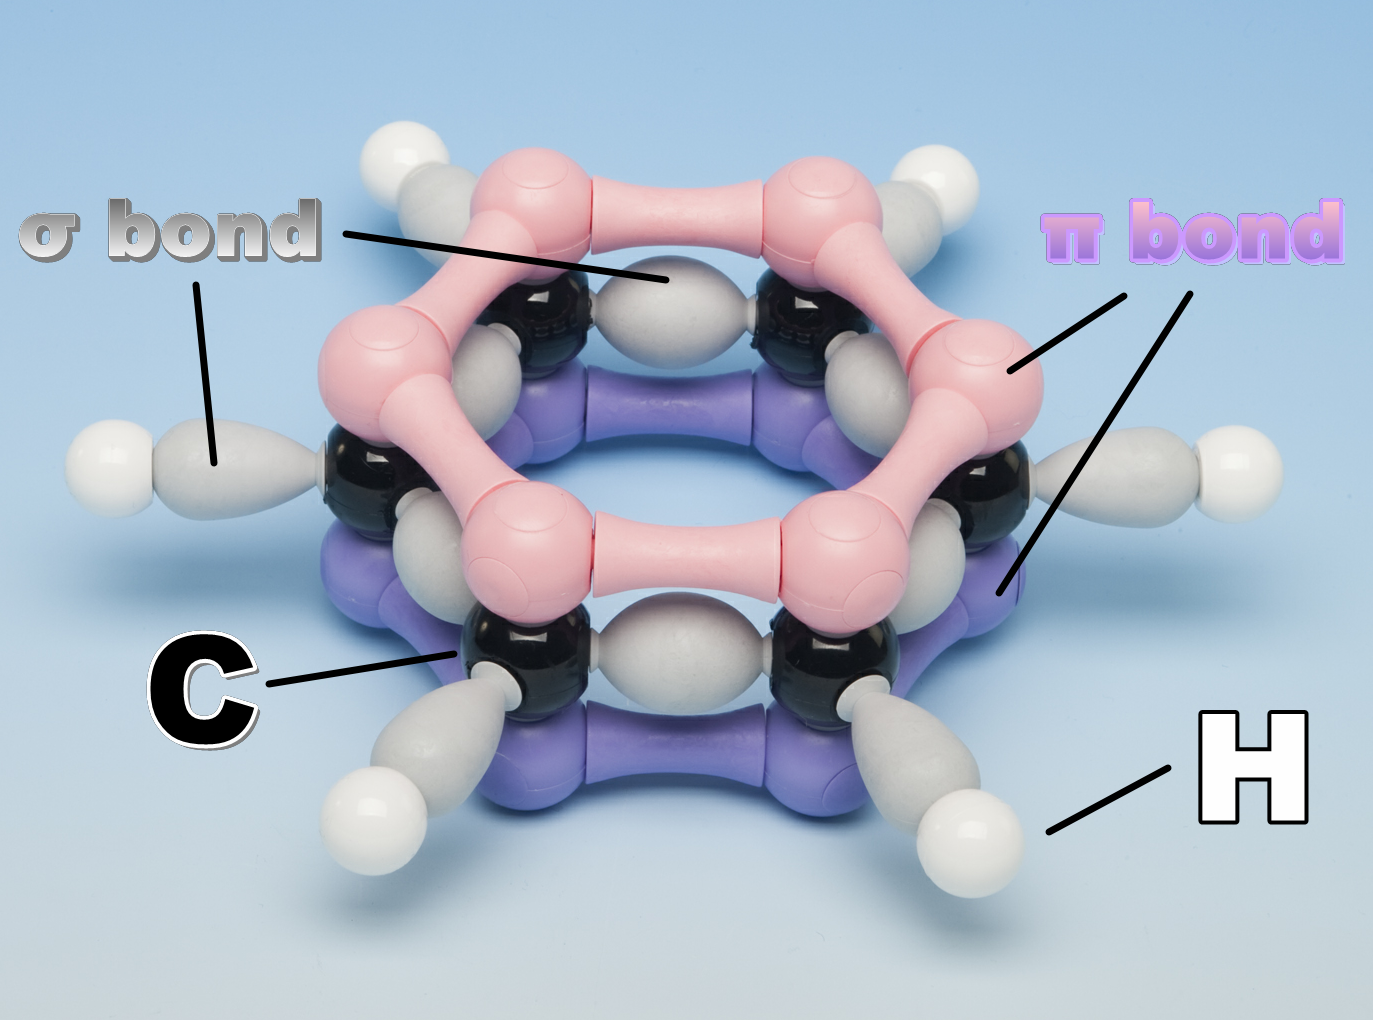
\includegraphics[width=7cm]{image/6-3-10.png}
\hspace{2cm}
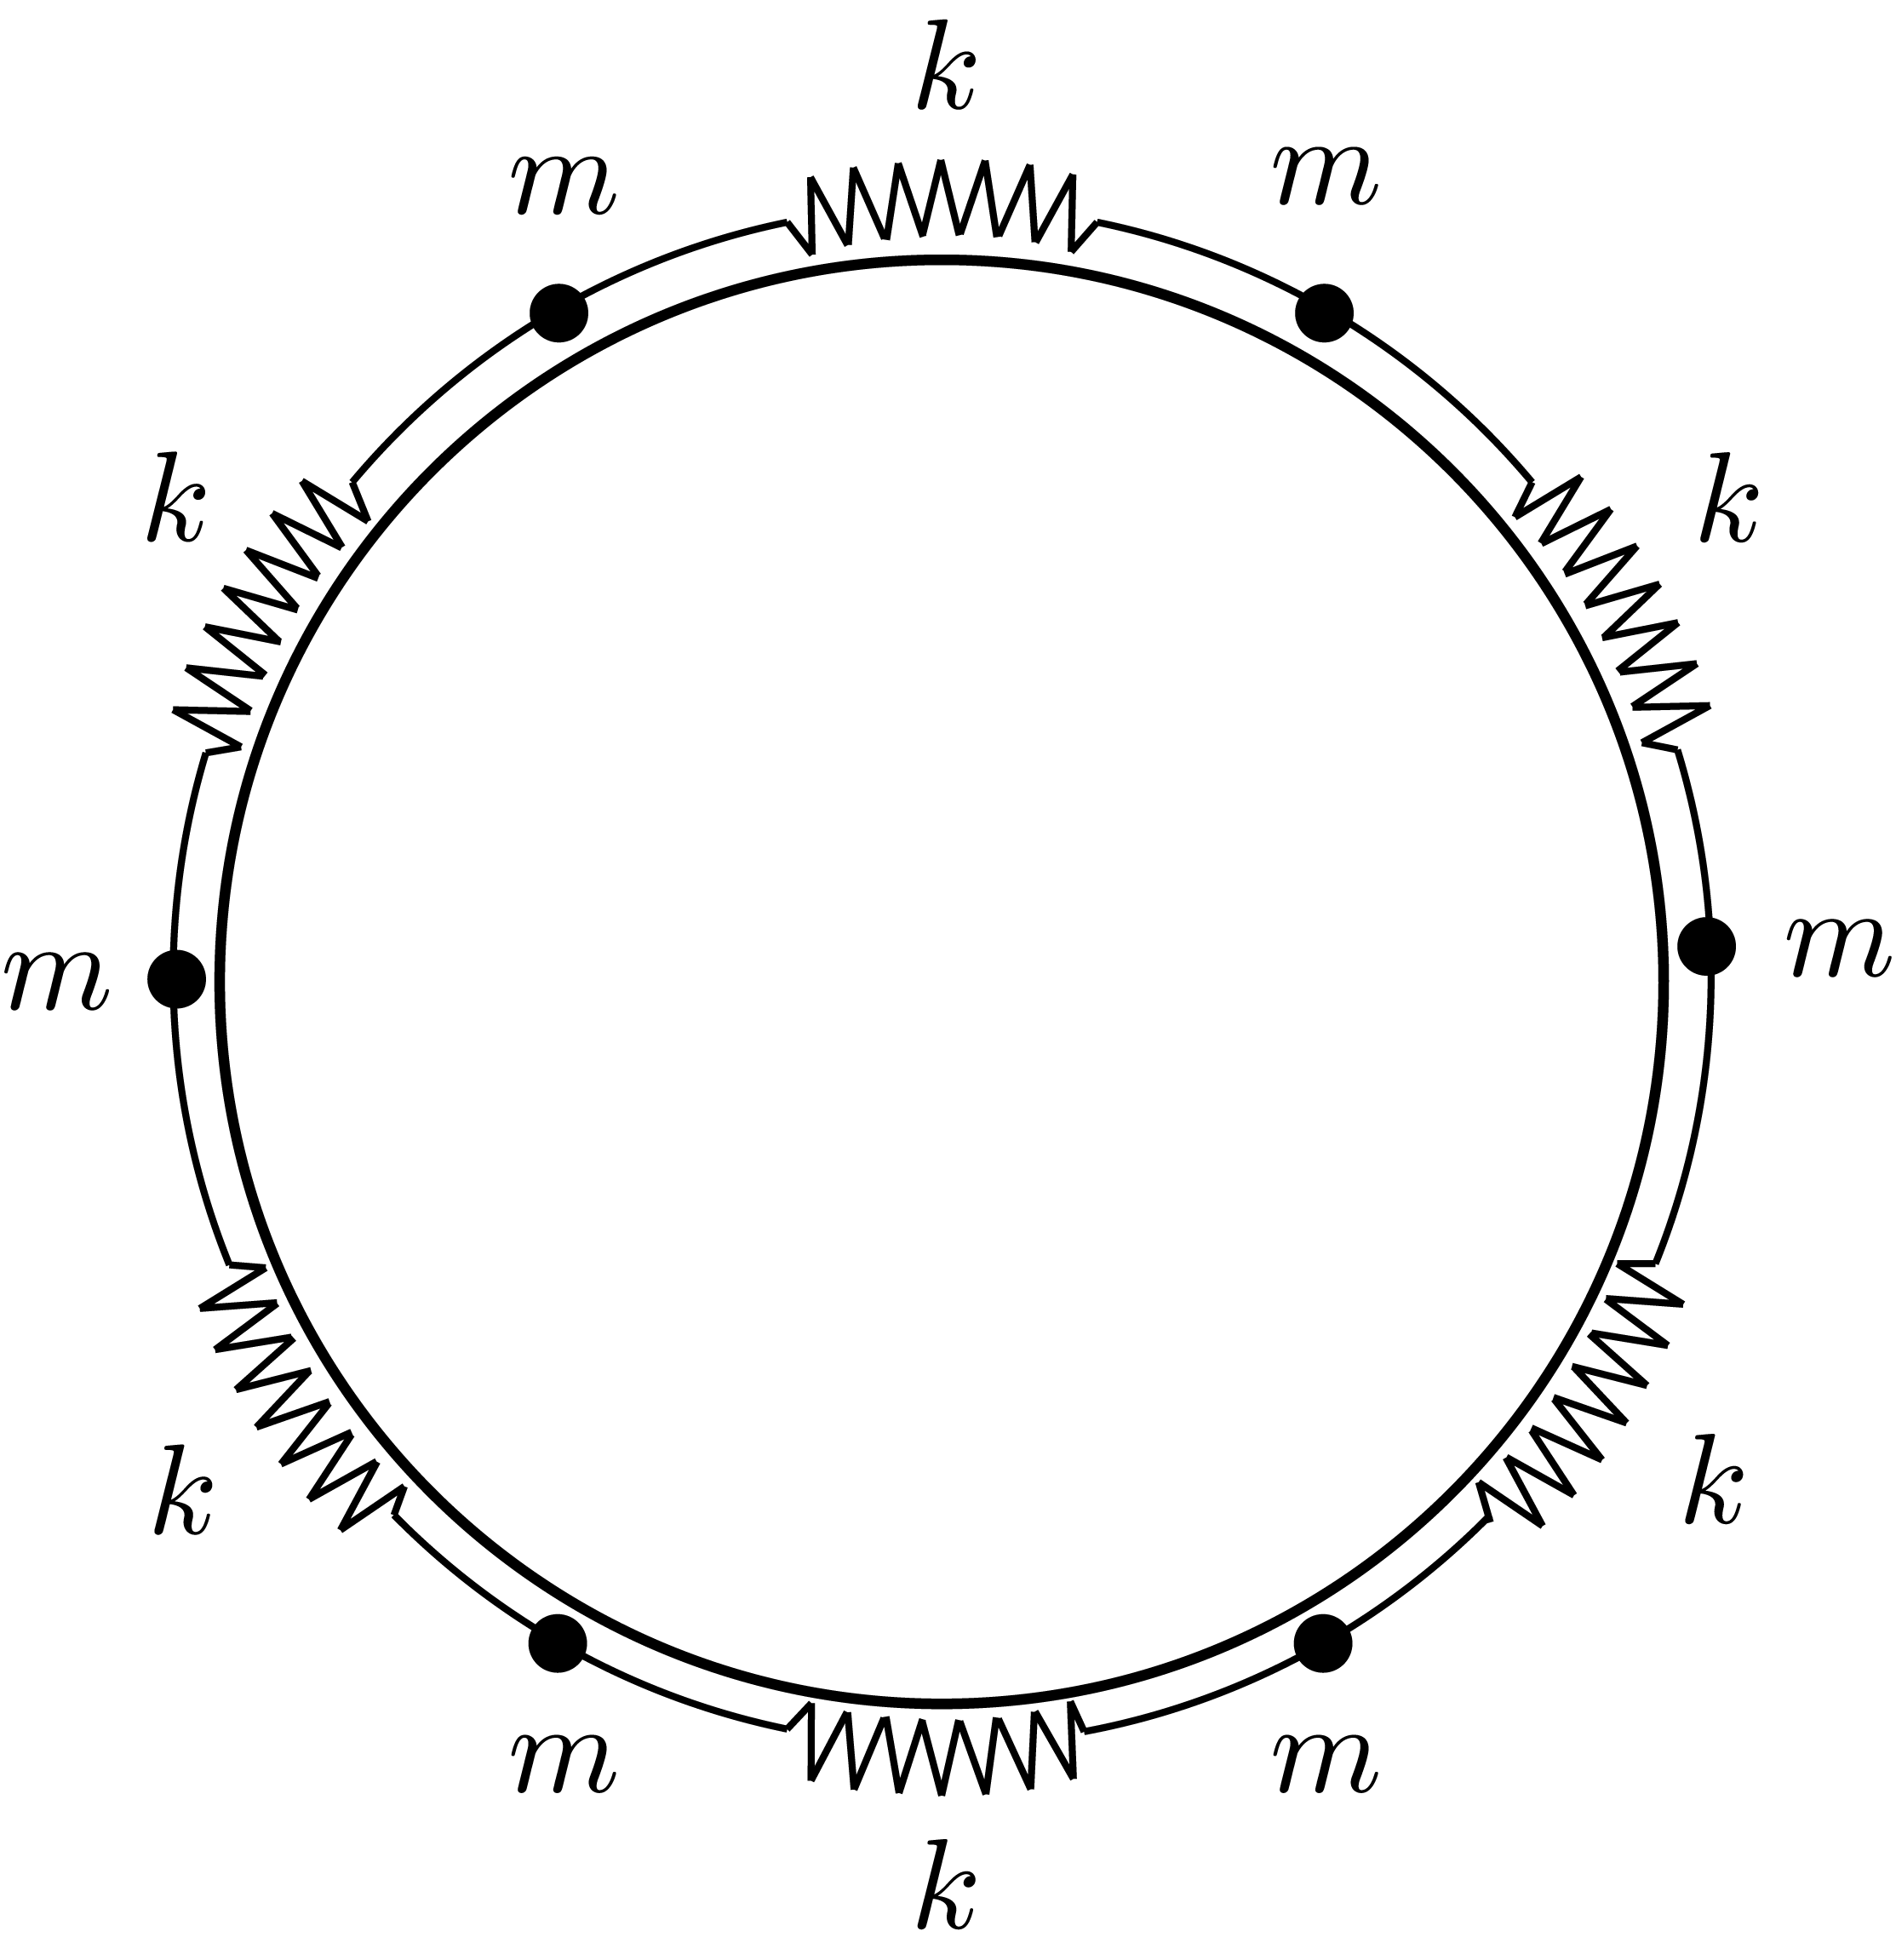
\includegraphics[width=5cm]{image/6-3-8.png}
\caption{苯: 6原子环问题}
\end{figure}

对于苯分子的振动光谱问题主要的部分就可以简化为$6$




\section{非线性摄动*}

\section{格波}



